%%% Hlavní soubor. Zde se definují základní parametry a odkazuje se na ostatní části. %%%

%% Verze pro jednostranný tisk:
% Okraje: levý 40mm, pravý 25mm, horní a dolní 25mm
% (ale pozor, LaTeX si sám přidává 1in)
\documentclass[12pt,a4paper]{report}

\newif\iffinal
\finalfalse

\setlength\textwidth{145mm}
\setlength\textheight{247mm}
\setlength\oddsidemargin{15mm}
\setlength\evensidemargin{15mm}
\setlength\topmargin{0mm}
\setlength\headsep{0mm}
\setlength\headheight{0mm}
% \openright zařídí, aby následující text začínal na pravé straně knihy
\let\openright=\clearpage

%% Pokud tiskneme oboustranně:
% \documentclass[12pt,a4paper,twoside,openright]{report}
% \setlength\textwidth{145mm}
% \setlength\textheight{247mm}
% \setlength\oddsidemargin{14.2mm}
% \setlength\evensidemargin{0mm}
% \setlength\topmargin{0mm}
% \setlength\headsep{0mm}
% \setlength\headheight{0mm}
% \let\openright=\cleardoublepage

%% Vytváříme PDF/A-2u
\usepackage[a-2u]{pdfx}

%% Přepneme na českou sazbu a fonty Latin Modern
%\usepackage[czech]{babel}
\usepackage[babelshorthands=false]{polyglossia}
\setmainlanguage{czech}
\setotherlanguages{english}
%\usepackage[T1]{fontenc}
%\usepackage{textcomp}

%% Použité kódování znaků: obvykle latin2, cp1250 nebo utf8:
% \usepackage[utf8]{inputenc}

%%% Další užitečné balíčky (jsou součástí běžných distribucí LaTeXu)
\usepackage{amsmath}        % rozšíření pro sazbu matematiky
\usepackage{amsfonts}       % matematické fonty
\usepackage{amsthm}         % sazba vět, definic apod.
\usepackage{bbding}         % balíček s nejrůznějšími symboly
% (čtverečky, hvězdičky, tužtičky, nůžtičky, ...)
\usepackage{bm}             % tučné symboly (příkaz \bm)
\usepackage{graphicx}       % vkládání obrázků
% width=\maxwidth{\textwidth}
\makeatletter
\def\maxwidth#1{\ifdim\Gin@nat@width>#1 #1\else\Gin@nat@width\fi}
\makeatother

\usepackage{fancyvrb}       % vylepšené prostředí pro strojové písmo
\usepackage{indentfirst}    % zavede odsazení 1. odstavce kapitoly
% \usepackage{natbib}         % zajištuje možnost odkazovat na literaturu
% stylem AUTOR (ROK), resp. AUTOR [ČÍSLO]

\usepackage[backend=biber,style=numeric,sorting=none]{biblatex}
\addbibresource{literatura.bib}

\usepackage[nottoc]{tocbibind} % zajistí přidání seznamu literatury,
% obrázků a tabulek do obsahu
% \usepackage{icomma}         % inteligetní čárka v matematickém módu
\usepackage{dcolumn}        % lepší zarovnání sloupců v tabulkách
\usepackage{booktabs}       % lepší vodorovné linky v tabulkách
\usepackage{paralist}       % lepší enumerate a itemize
\usepackage{xcolor}         % barevná sazba
\usepackage[shortlabels]{enumitem}
\usepackage{makecell}
% nice typesetting of keyboard keys, shortcuts, and file paths
\usepackage[os=win]{menukeys}

%%%% TIKZ
\usepackage{tikz}
\usetikzlibrary{positioning}
\usetikzlibrary{shapes.geometric}
\usetikzlibrary{arrows}
\usepackage{tikz-cd}
%%%% END TIKZ

\usepackage{array}
\usepackage{caption}
\usepackage{subcaption}
\usepackage{xargs} % Use more than one optional parameter in new commands

% Make "quotes" typeset the Czech ,,quotes''
\usepackage{csquotes}
\MakeOuterQuote{"}

%%%% TODO notes
\iffinal
\newcommandx{\unsure}[2][1=]{}
\newcommandx{\change}[2][1=]{}
\newcommandx{\info}[2][1=]{}
\newcommandx{\improvement}[2][1=]{}
\newcommandx{\missingfigure}[2][1=]{Chybí obrázek}
\else
\usepackage[colorinlistoftodos,prependcaption,textsize=tiny]{todonotes}
\newcommandx{\unsure}[2][1=]{\todo[linecolor=red,backgroundcolor=red!25,bordercolor=red,#1]{#2}}
\newcommandx{\change}[2][1=]{\todo[linecolor=blue,backgroundcolor=blue!25,bordercolor=blue,#1]{#2}}
\newcommandx{\info}[2][1=]{\todo[linecolor=OliveGreen,backgroundcolor=OliveGreen!25,bordercolor=OliveGreen,#1]{#2}}
\newcommandx{\improvement}[2][1=]{\todo[linecolor=Plum,backgroundcolor=Plum!25,bordercolor=Plum,#1]{#2}}
\newcommandx{\thiswillnotshow}[2][1=]{\todo[disable,#1]{#2}}
\paperwidth=\dimexpr \paperwidth + 6cm\relax
\oddsidemargin=\dimexpr\oddsidemargin + 3cm\relax
\evensidemargin=\dimexpr\evensidemargin + 3cm\relax
\marginparwidth=\dimexpr \marginparwidth + 3cm\relax
\fi
%%%% END TODO notes

%%%% Listings
\usepackage{listings}
\renewcommand{\lstlistingname}{Kód}
\definecolor{codegreen}{rgb}{0,0.6,0}
\definecolor{codegray}{rgb}{0.5,0.5,0.5}
\definecolor{codepurple}{rgb}{0.58,0,0.82}
\definecolor{backcolor}{rgb}{0.95,0.95,0.92}
\lstdefinestyle{mystyle}{
  backgroundcolor=\color{backcolor},
  commentstyle=\color{codegreen},
  keywordstyle=\color{magenta},
  numberstyle=\tiny\color{codegray},
  stringstyle=\color{codepurple},
  basicstyle=\ttfamily\footnotesize,
  breakatwhitespace=false,
  breaklines=true,
  captionpos=b,
  keepspaces=true,
  numbers=left,
  numbersep=5pt,
  showspaces=false,
  showstringspaces=false,
  showtabs=false,
  tabsize=2
}
\lstset{style=mystyle}
%%%% END Listings

% better hyphenation, use \hyp{} to suggest hyphen
\usepackage{hyphenat}

%%%% FONT
\usepackage{lmodern}
% Use sans-serif in captions and floats (figures, tables)
\usepackage{caption}
\usepackage[font=sf]{floatrow}
% this package provides a serif, sans, and mono font
% the T1 version does not result in a correct pdf/a-2u
\usepackage[mono=true]{libertinus-otf} % popular for comp-sci (ACM uses this)
%\usepackage{tgschola} % Schoolbook-like (gives a bit of historic feel)
% better typography resulting in better justification, less overfull hboxes, and overall nicer document.
\usepackage{microtype}
%%%% END FONT

%%%% convenience commands
\newcommand{\xmark}{\XSolidBrush}
\newcommand{\cmark}{\CheckmarkBold}
\newcommand{\set}[1]{\left\{#1\right\}}
\newcommand{\zero}{\texttt{0}}
\newcommand{\one}{\texttt{1}}
\newcommand{\many}{\texttt{*}}
%%%% end convenience commands

%%% Údaje o práci

% Název práce v jazyce práce (přesně podle zadání)
\def\NazevPrace{\input{metadata/title-cz.txt}}

% Název práce v angličtině
\def\NazevPraceEN{\input{metadata/title-en.txt}}

% Jméno autora
\def\AutorPrace{Dennis Pražák}

% Rok odevzdání
\def\RokOdevzdani{2023}

% Název katedry nebo ústavu, kde byla práce oficiálně zadána
% (dle Organizační struktury MFF UK, případně plný název pracoviště mimo MFF)
\def\Katedra{Katedra softwarového inženýrství}
\def\KatedraEN{Department of Software Engineering}

% Jedná se o katedru (department) nebo o ústav (institute)?
\def\TypPracoviste{Katedra}
\def\TypPracovisteEN{Department}

% Vedoucí práce: Jméno a příjmení s~tituly
\def\Vedouci{RNDr.~Martin Svoboda, Ph.D.}

% Pracoviště vedoucího (opět dle Organizační struktury MFF)
\def\KatedraVedouciho{\Katedra}
\def\KatedraVedoucihoEN{\KatedraEN}

% Studijní program a obor
\def\StudijniProgram{Informatika }
\def\StudijniObor{IPP2}

% Nepovinné poděkování (vedoucímu práce, konzultantovi, tomu, kdo
% zapůjčil software, literaturu apod.)
\def\Podekovani{%
  Děkuji vedoucímu RNDr.~Martinu Svobodovi,~PhD., za odborné vedení práce a všechny poskytnuté rady a podněty.
}

% Abstrakt (doporučený rozsah cca 80-200 slov; nejedná se o zadání práce)
\def\Abstrakt{%%% Šablona pro jednoduchý soubor formátu PDF/A, jako treba samostatný abstrakt práce.

\documentclass[12pt]{report}

\usepackage[a4paper, hmargin=1in, vmargin=1in]{geometry}
\usepackage[a-2u]{pdfx}
\usepackage{polyglossia}
\setmainlanguage{czech}
\setotherlanguages{english}
\usepackage{lmodern}
\usepackage{textcomp}
\usepackage{microtype}
\usepackage[mono=true]{libertinus-otf}

\begin{document}

%%% Šablona pro jednoduchý soubor formátu PDF/A, jako treba samostatný abstrakt práce.

\documentclass[12pt]{report}

\usepackage[a4paper, hmargin=1in, vmargin=1in]{geometry}
\usepackage[a-2u]{pdfx}
\usepackage{polyglossia}
\setmainlanguage{czech}
\setotherlanguages{english}
\usepackage{lmodern}
\usepackage{textcomp}
\usepackage{microtype}
\usepackage[mono=true]{libertinus-otf}

\begin{document}

\input{metadata/abstrakt-cz.txt}

\end{document}


\end{document}
}
\def\AbstraktEN{%%% Šablona pro jednoduchý soubor formátu PDF/A, jako treba samostatný abstrakt práce.

\documentclass[12pt]{report}

\usepackage[a4paper, hmargin=1in, vmargin=1in]{geometry}
\usepackage[a-2u]{pdfx}
\usepackage{polyglossia}
\setmainlanguage{czech}
\setotherlanguages{english}
\usepackage{lmodern}
\usepackage{textcomp}
\usepackage{microtype}
\usepackage[mono=true]{libertinus-otf}

\begin{document}

%%% Šablona pro jednoduchý soubor formátu PDF/A, jako treba samostatný abstrakt práce.

\documentclass[12pt]{report}

\usepackage[a4paper, hmargin=1in, vmargin=1in]{geometry}
\usepackage[a-2u]{pdfx}
\usepackage{polyglossia}
\setmainlanguage{czech}
\setotherlanguages{english}
\usepackage{lmodern}
\usepackage{textcomp}
\usepackage{microtype}
\usepackage[mono=true]{libertinus-otf}

\begin{document}

\input{metadata/abstrakt-en.txt}

\end{document}


\end{document}
}

% 3 až 5 klíčových slov (doporučeno), každé uzavřeno ve složených závorkách
\def\KlicovaSlova{\input{metadata/keywords-cz.txt}}
\def\KlicovaSlovaEN{\input{metadata/keywords-en.txt}}


%% Balíček hyperref, kterým jdou vyrábět klikací odkazy v PDF,
%% ale hlavně ho používáme k uložení metadat do PDF (včetně obsahu).
%% Většinu nastavítek přednastaví balíček pdfx.
\hypersetup{unicode}
\hypersetup{breaklinks=true}
\usepackage{xurl}

%% Definice různých užitečných maker (viz popis uvnitř souboru)
%%% Tento soubor obsahuje definice různých užitečných maker a prostředí %%%
%%% Další makra připisujte sem, ať nepřekáží v ostatních souborech.     %%%

%%% Drobné úpravy stylu

% Tato makra přesvědčují mírně ošklivým trikem LaTeX, aby hlavičky kapitol
% sázel příčetněji a nevynechával nad nimi spoustu místa. Směle ignorujte.
\makeatletter
\def\@makechapterhead#1{
  {\parindent \z@ \raggedright \normalfont
   \Huge\bfseries \thechapter. #1
   \par\nobreak
   \vskip 20\p@
}}
\def\@makeschapterhead#1{
  {\parindent \z@ \raggedright \normalfont
   \Huge\bfseries #1
   \par\nobreak
   \vskip 20\p@
}}
\makeatother

% Custom -- úprava mezer řádků
\setlength{\parskip}{0.2em}
\setlist[enumerate]{partopsep=\parskip, topsep=\parskip, itemsep=0pt}
\setlist[itemize]{partopsep=\parskip, topsep=\parskip, itemsep=0pt}

% Toto makro definuje kapitolu, která není očíslovaná, ale je uvedena v obsahu.
\def\chapwithtoc#1{
\chapter*{#1}
\addcontentsline{toc}{chapter}{#1}
}

% Trochu volnější nastavení dělení slov, než je default.
\lefthyphenmin=2
\righthyphenmin=2

\iffinal
\else
% Zapne černé "slimáky" na koncích řádků, které přetekly, abychom si
% jich lépe všimli.
\overfullrule=1mm
\fi

%%% Makra pro definice, věty, tvrzení, příklady, ... (vyžaduje baliček amsthm)

\theoremstyle{plain}
\newtheorem{veta}{Věta}
\newtheorem{lemma}[veta]{Lemma}
\newtheorem{tvrz}[veta]{Tvrzení}

\theoremstyle{plain}
\newtheorem{definice}{Definice}

\theoremstyle{remark}
\newtheorem*{dusl}{Důsledek}
\newtheorem*{pozn}{Poznámka}
\newtheorem*{prikl}{Příklad}

%%% Prostředí pro důkazy

\newenvironment{dukaz}{
  \par\medskip\noindent
  \textit{Důkaz}.
}{
\newline
\rightline{$\qedsymbol$}
}

%%% Prostředí pro sazbu kódu, případně vstupu/výstupu počítačových
%%% programů. (Vyžaduje balíček fancyvrb -- fancy verbatim.)

\DefineVerbatimEnvironment{code}{Verbatim}{fontsize=\small, frame=single}

%%% Prostor reálných, resp. přirozených čísel
\newcommand{\R}{\mathbb{R}}
\newcommand{\N}{\mathbb{N}}

%%% Užitečné operátory pro statistiku a pravděpodobnost
\DeclareMathOperator{\pr}{\textsf{P}}
\DeclareMathOperator{\E}{\textsf{E}\,}
\DeclareMathOperator{\var}{\textrm{var}}
\DeclareMathOperator{\sd}{\textrm{sd}}

%%% Příkaz pro transpozici vektoru/matice
\newcommand{\T}[1]{#1^\top}

%%% Vychytávky pro matematiku
\newcommand{\goto}{\rightarrow}
\newcommand{\gotop}{\stackrel{P}{\longrightarrow}}
\newcommand{\maon}[1]{o(n^{#1})}
\newcommand{\abs}[1]{\left|{#1}\right|}
\newcommand{\dint}{\int_0^\tau\!\!\int_0^\tau}
\newcommand{\isqr}[1]{\frac{1}{\sqrt{#1}}}

%%% Vychytávky pro tabulky
\newcommand{\pulrad}[1]{\raisebox{1.5ex}[0pt]{#1}}
\newcommand{\mc}[1]{\multicolumn{1}{c}{#1}}

%% Dočasná implementace pro zkratky
% \newacronym{gcd}{GCD}{Greatest Common Divisor}, \acrshort{gcd}
\newcommand{\newacronym}[3]{%
  \expandafter\newcommand\csname acrshort#1\endcsname{#2}%
  \expandafter\newcommand\csname acrlong#1\endcsname{#3}%
}
\newcommand{\acrshort}[1]{\csname acrshort#1\endcsname}
\newcommand{\acrlong}[1]{\csname acrlong#1\endcsname}
\newcommand{\acrfull}[1]{\csname acrlong#1\endcsname\ (\csname acrshort#1\endcsname)}


%% Titulní strana a různé povinné informační strany
\begin{document}
% \title{\NazevPrace}
% \author{\AutorPrace}
% \date{Draft \today}

%%% Titulní strana práce a další povinné informační strany

%%% Titulní strana práce

\pagestyle{empty}
\hypersetup{pageanchor=false}

\begin{center}

\centerline{\mbox{
\includegraphics[width=166mm]{../img/logo-cs.pdf}}}

\vspace{-8mm}
\vfill

{\bf\Large BAKALÁŘSKÁ PRÁCE}

\vfill

{\LARGE\AutorPrace}

\vspace{15mm}

{\LARGE\bfseries\NazevPrace}

\vfill

\Katedra

\vfill

{
\centerline{\vbox{\halign{\hbox to 0.45\hsize{\hfil #}&\hskip 0.5em\parbox[t]{0.45\hsize}{\raggedright #}\cr
Vedoucí bakalářské práce:&\Vedouci \cr
\noalign{\vspace{2mm}}
Studijní program:&\StudijniProgram \cr
\noalign{\vspace{2mm}}
Studijní obor:&\StudijniObor \cr
}}}}

\vfill

% Zde doplňte rok
Praha \RokOdevzdani

\end{center}

\newpage

%%% Následuje vevázaný list -- kopie podepsaného "Zadání bakalářské práce".
%%% Toto zadání NENÍ součástí elektronické verze práce, nescanovat.

%%% Strana s čestným prohlášením k bakalářské práci

\openright
\hypersetup{pageanchor=true}
\pagestyle{plain}
\pagenumbering{roman}
\vglue 0pt plus 1fill

\noindent
Prohlašuji, že jsem tuto bakalářskou práci vypracoval(a) samostatně a výhradně
s~použitím citovaných pramenů, literatury a dalších odborných zdrojů.
Tato práce nebyla využita k~získání jiného nebo stejného titulu.

\medskip\noindent
Beru na~vědomí, že se na moji práci vztahují práva a povinnosti vyplývající
ze zákona č. 121/2000 Sb., autorského zákona v~platném znění, zejména skutečnost,
že Univerzita Karlova má právo na~uzavření licenční smlouvy o~užití této
práce jako školního díla podle §60 odst. 1 autorského zákona.

\vspace{10mm}

\hbox{\hbox to 0.5\hsize{%
V~\hbox to 6em{\dotfill} dne \hbox to 6em{\dotfill}
\hss}\hbox to 0.5\hsize{\dotfill\quad}}
\smallskip
\hbox{\hbox to 0.5\hsize{}\hbox to 0.5\hsize{\hfil Podpis autora\hfil}}

\vspace{20mm}
\newpage

%%% Poděkování

\openright

\noindent
\Podekovani

\newpage

%%% Povinná informační strana bakalářské práce

\openright

\vbox to 0.5\vsize{
\setlength\parindent{0mm}
\setlength\parskip{5mm}

Název práce:
\NazevPrace

Autor:
\AutorPrace

\TypPracoviste:
\Katedra

Vedoucí bakalářské práce:
\Vedouci, \KatedraVedouciho

Abstrakt:
\Abstrakt

Klíčová slova:
\KlicovaSlova

\vss}\nobreak\vbox to 0.49\vsize{
\setlength\parindent{0mm}
\setlength\parskip{5mm}

Title:
\NazevPraceEN

Author:
\AutorPrace

\TypPracovisteEN:
\KatedraEN

Supervisor:
\Vedouci, \KatedraVedoucihoEN

Abstract:
\AbstraktEN

Keywords:
\KlicovaSlovaEN

\vss}

\newpage

\openright
\pagestyle{plain}
\pagenumbering{arabic}
\setcounter{page}{1}


%%% Strana s automaticky generovaným obsahem bakalářské práce

\tableofcontents

%%% Jednotlivé kapitoly práce jsou pro přehlednost uloženy v samostatných souborech
% \chapter*{Úvod}
\addcontentsline{toc}{chapter}{Úvod}

\todotext{Úvod}

% \chapter{Existující nástroje}

V~této kapitole zanalyzujeme některé existující nástroje pro tvorbu diagramů a~porovnáme je dle navržených kritérií.
Všechny analyzované nástroje jsou dostupné online ve webovém prohlížeči, jelikož v~praktické části bude implementován nástroj pro stejné prostředí.
Nástroji, které budeme porovnávat, jsou
\begin{itemize}
  \item diagrams.net~\cite{drawio_2023} vhodné pro tvorbu libovolných diagramů,
  \item drawSQL~\cite{drawsql_2021} určené pro tvorbu relačních schémat,
  \item ERDPlus~\cite{erdplus_2023} k~vytváření zejména ER diagramů~\cite{chen_er_1976}.
  \item nomnoml~\cite{nomnoml_2022} k~tvorbě UML diagramů~\cite{omg_uml_2017} psaním textu,
  \item Visual Paradigm Online~\cite{vpo_2022} pro tvorbu libovolných diagramů.
\end{itemize}

Před představením existujících nástrojů určíme srovnávací kritéria, dle kterých budeme nástroje analyzovat.

\section{Srovnávací kritéria}

Prvním kritériem pro porovnání nástrojů je jejich kategorie, která vypovídá o~účelu nástroje a~cílové skupině zákazníků.
Základní kategorie jsou
\begin{itemize}
  \item konceptuální vrstva -- tyto nástroje jsou většinou určené pro tvorbu ER diagramů, případně jiným způsobem modelují vztahy a~atributy entit, na které při datovém modelování vymezujeme svůj diskurz,
  \item logická (též technologická) vrstva -- tyto nástroje umožňují tvorbu diagramů s~ohledem na typ struktur, v~kterých jsou data uchovávána, např. relační databáze,
  \item kresba libovolných diagramů -- nástroje, které nejsou omezeny téměř žádným standardem či konvencí a~umožňují kresbu libovolných diagramů,
  \item kresba omezených diagramů -- nástroje, které umožňují kresbu diagramů omezených na existující schémata (ER, UML, \dots).
\end{itemize}

Dalším kritériem je typ úložiště.
Nástroje mohou ukládat svá data do paměti prohlížeče (lokálně pro uživatele), na své servery, nebo používat externí úložiště uživatele, například Google Drive\footnote{\url{https://www.google.com/drive/}}.
Čím více různých typů úložiště nástroj podporuje, tím lépe, neboť uživatel může flexibilně zvolit jeho účelům vyhovující způsob uchovávání dat.
Pro interaktivní spolupráci s~týmem je lepší sdílené úložiště a~pro lokální práci je vhodnější lokální úložiště.

Interaktivní spolupráce je dalším důležitým kritériem.
U~velkých projektů je vývoj modelu urychlen, pokud nástroj spolupráci umožňuje.

Dále budeme porovnávat formát, do kterého nástroj diagram ukládá (pokud k~uloženému souboru má uživatel přístup).
Může se jednat o~serializovaný dokument do dobře známého standardního formátu, nebo o~vlastní formát, který je často nakonec také založený na nějakém standardu.

Kromě uložení rozdělané práce do vhodného formátu musí nástroj umožnit export do formátu, který uživatelé využijí pro své účely.
Formáty pro export lze rozdělit do několika kategorií:
\begin{itemize}
  \item serializovaný formát -- většinou se jedná o~vlastní formát aplikace a~takový soubor nelze jinou aplikací otevřít, ale lze jej programově zpracovat,
  \item rastrové formáty, např. \acrfull{png}\footnote{Portable Network Graphics -- \url{https://www.w3.org/TR/2003/REC-PNG-20031110/}} -- mají nejširší využití a~podporu, lze je použít v~dokumentech a~na webových stránkách,
  \item vektorové formáty, např. \acrfull{svg}~\cite{brinza_svg_2018} -- nemají tak rozšířenou podporu, nicméně jsou vhodnější v~dokumentech po estetické stránce (zvlášť při tištění);
        dále existují vektorové editory, pomocí nichž lze výsledek libovolně upravovat bez potřeby souboru ve serializovaném formátu;
        většina webových prohlížečů formát \acrshort{svg} podporuje a~soubor vykreslí;
        do této kategorie lze zařadit i~jiné otevřené strukturované formáty, např. VSDX\footnote{Microsoft Visio XML formát založený na ISO 29500 -- \url{https://interoperability.blob.core.windows.net/files/MS-VSDX/\%5bMS-VSDX\%5d.pdf}},
  \item zjednodušený export -- některé nástroje šetří práci uživatele tím, že diagram rovnou exportují do HTML\footnote{HyperText Markup Language -- \url{https://w3.org/TR/2021/SPSD-html52-20210128/}}, PDF\footnote{Portable Document Format, ISO 32000 -- \url{https://iso.org/standard/75839.html}} a~podobných finálních formátů pro okamžitou aplikaci, přestože uživatel může zvolit jiný formát a~finální vytvořit sám,
  \item schematické formáty, např. SQL\footnote{Structured Query Language -- \url{https://iso.org/standard/63555.html}} -- téměř výhradně u~nástrojů lo\-gic\-ké vrst\-vy; umožňují rovnou vytvářet schémata pro databáze.
\end{itemize}

Stejně jako u~typu úložiště, čím více různých formátů exportu nástroj podporuje, tím lépe, neboť nástroj je flexibilní.

Posledním, neméně důležitým kritériem, je způsob komercializace.
Většina volně dostupných nástrojů je nějakým způsobem zpoplatněna, ať už se jedná o~jednorázový nebo pravidelný poplatek.
Nejčastějším komerčním modelem je verze zdarma s~omezenými funkcemi a~dále několik placených plánů různé úrovně s~odemčenými pokročilými funkcemi.
U~tohoto modelu je důležité vyrovnat funkce tak, aby byl nástroj použitelný i~v~bezplatné verzi, a~aby byly placené funkce atraktivní pro uživatele.
Při srovnávání budeme věnovat pozornost i~tomu, jestli jsou placené funkce esenciální.

\section{draw.io}\label{section:drawio}

Srovnávací kritéria:
\begin{itemize}
  \item kategorie -- kresba libovolných diagramů,
  \item typ úložiště -- lokální, externí, prohlížeč,
  \item export -- serializovaný, rastrový, vektorový, zjednodušený,
  \item interaktivní spolupráce -- částečně podporována (pomocí externích úložišť),
  \item komercializace -- veškeré funkce jsou zdarma a~není potřeba uživatelský účet;
        z~jiného pohledu lze počítat cenu externích úložišť, ale ta jsou volitelná.
\end{itemize}

Nástroj diagrams.net~\cite{drawio_2023}, dříve draw.io, je obecný open-source kreslící nástroj
(který však nepřijímá změny od externích vývojářů~\cite{drawio_gh_2022}) % https://github.com/jgraph/drawio/blob/c7122cad617f52563c11d90890e64ab06db3a27a/README.md#open-source-not-open-contribution
vydaný s~licencí Apache License 2.0\footnote{\url{https://www.apache.org/licenses/LICENSE-2.0}}, dostupný jako webová aplikace\footnote{na adrese \url{https://app.diagrams.net}} nebo jako desktopová aplikace.
Desktopová verze aplikace je sestavena stejným způsobem jako webová, pouze je zabalena pomocí platformy Electron~\cite{openjsfoundation_electron_2023} do okna Chromium.
Je vyvinut v~běžných we\-bo\-vých tech\-no\-lo\-gi\-ích (Java\-Script\footnote{Standardizován jako ECMAScript, ISO 16262 -- \url{https://iso.org/standard/55755.html}}, CSS\footnote{Cascading Style Sheets -- \url{https://www.w3.org/TR/css}}, HTML).

Diagramy lze uložit do serializovaného XML\footnote{Extensible Markup Language -- \url{https://www.w3.org/TR/xml/}} formátu \texttt{.drawio}.
V~tomto formátu je pro každý diagram XML element \texttt{diagram}, ve kterém se nachází data zakódována do Base64\footnote{RFC 2045 \S6.8 -- \url{https://datatracker.ietf.org/doc/html/rfc2045\#section-6.8}}.
Tato data jsou komprimována pomocí zlib\footnote{\url{https://zlib.net}} a~obsahují další XML dokument (URL-encoded\footnote{RFC 3986 \S2.1 -- \url{https://datatracker.ietf.org/doc/html/rfc3986\#section-2.1}}, tj. zakódovaný), tentokrát již serializaci vlastního diagramu~\cite{seibert_extractingxml_2016}.
Formát tak není bez dekomprese čitelný člověkem.
Výhodou je, že lze uložit více diagramů do jednoho souboru a~každý pojmenovat.
Rozhraní k~tomu určené je identické s~listy souboru tabulkových procesorů, jako Microsoft Excel\footnote{\url{https://aka.ms/excel}} a~Google Sheets\footnote{\url{https://sheets.google.com}}.

Jednosouborový program v~jazyce Python (viz kód~\ref{code:mxfiledec}) přijímá na standardním vstupu base64 řetězec formátu mxfile a na standardní výstup vypíše výslednou dekódovanou XML serializaci.
Použití algoritmu Inflate na syrová data je vynuceno podle dokumentace zlib\footnote{\url{https://www.zlib.net/manual.html}}.
% specificky https://www.zlib.net/manual.html#:~:text=windowbits%20can%20also%20be%20%E2%80%938..%E2%80%9315%20for%20raw%20deflate
Jedná se o~ukázku postupu dekódování a toho, že formát je otevřený.
Organizace JGraph dokonce poskytuje online nástroj\footnote{k dispozici na adrese \url{https://jgraph.github.io/drawio-tools/tools/convert.html}}, pomocí kterého lze dosáhnout téhož výsledku.

Soubor s~diagramy lze také uložit do formátu \acrshort{svg}, který je navíc otevřený a~podporují ho jiné nástroje.
Uživatel má při exportu k~dispozici možnost \textit{Include a~copy of my diagram}, která do \acrshort{svg} souboru zahrne již zmíněný Base64 řetězec, ve kterém je diagram serializovaný.
Ve výsledku to znamená, že takto exportované \acrshort{svg} soubory umí diagrams.net i~otevřít a~práce na nich může plnohodnotně pokračovat.
Toto řešení se nám líbí, protože se jedná o~schování vlastního formátu do \acrshort{svg}, který je nejvhodnějším pro přechovávání a~zobrazování diagramů.

\begin{lstlisting}[language=Python, caption=Dekódování mxfile, label=code:mxfiledec, float=htb]
from sys import stdin
from base64 import b64decode
from zlib import decompress, MAX_WBITS
from urllib.parse import unquote

base64_data = stdin.read()
deflated_data = b64decode(base64_data, validate=False)
# wbits must be -MAX_WBITS which makes zlib use the raw Inflate algorithm without header detection
urlencoded_inflated_data = decompress(deflated_data, -MAX_WBITS)
urldecoded_data = unquote(urlencoded_inflated_data)
print(urldecoded_data)
\end{lstlisting}

Dalšími možnostmi exportu a~ukládání jsou
\begin{itemize}
  \item rastrové soubory \acrshort{png}, JPEG\footnote{Joint Photographic Experts Group, ISO 19566 -- \url{https://iso.org/standard/65348.html}},
  \item soubor PDF, do kterého je ve vektorovém formátu diagram vložen,
  \item soubor HTML, do kterého lze podobně jako v~\acrshort{svg} data diagramu uložit v~serializované formě, případně pouze vložit veřejný odkaz URL na diagram (pokud je použito odpovídající úložiště);
        v~tomto souboru je pak zahrnut JavaScript od diagrams.net, který diagram vykreslí,
  \item otevřený formát VSDX, původně vyvinutý pro Microsoft Visio.
\end{itemize}

Zajímavou vlastností exportu do rastrového formátu \acrshort{png} je, že po otevření v~programu diagrams.net je diagram plnohodnotně upravovatelný.
Je toho dosaženo tím, že v~\texttt{tEXt} chunku\footnote{dle \acrshort{png} formátu sekce 11.3.4.3 \url{https://www.w3.org/TR/2003/REC-PNG-20031110/}}
je pod klíčovým slovem \texttt{mxfile} zahrnuta plnohodnotná serializace diagramu.

Ze stejných souborů lze diagramy také importovat, ovšem editovat je lze jen pokud je v~nich zahrnut formát drawio, čehož je dosaženo u~některých formátů popsaných výše.

Jako úložiště si lze vybrat Google Drive,
OneDrive\footnote{\url{https://aka.ms/onedrive}},
Dropbox\footnote{\url{https://dropbox.com}},
GitHub\footnote{\url{https://github.com}},
Git\-Lab\footnote{\url{https://gitlab.com}},
paměť prohlížeče a~místní úložiště (disk uživatele).
Soubor lze ze stejných úložišť i~otevřít a~importovat, navíc k~tomu i~z~libovolné dostupné URL.

Interaktivní spolupráce je umožněna pouze pokud soubor jako úložiště využívá takové, ke kterému mají přístup zápisu (popř. pouze čtení) všichni účastnící se uživatelé (Google Drive, OneDrive, Dropbox, GitHub, GitLab).
Tato úložiště je však nutno manuálně vhodně nastavit (přístup ostatním uživatelům).
U~všech úložišť je rychlost reflektování změn ostatních uživatelů podobná -- vcelku pomalá, protože aplikace musí změny aktivně kontrolovat a~načítat.

Menu \menu{File > Publish} chybně napovídá, že se jedná o~funkci interaktivní spolupráce.
Ve skutečnosti je uživateli jen zobrazen odkaz na soubor ve vybraném úložišti (ale pouze pro Google Drive a~OneDrive, jinak je tato možnost vypnuta).
Spolupracující uživatel tak musí tento soubor v~daném úložišti uložit k~sobě (sdíleně), aby mohla spolupráce začít.

Jako další možnost jsme zvažovali desktopovou aplikaci s~načteným souborem, který je libovolným externím nástrojem sdílen mezi uživateli.
Soubor se nepřenačítá automaticky, ale musí být manuálně synchronizován tlačítkem \menu{File > Synchronize}, které je dostupné pouze v~desktopové verzi aplikace.
Uživatel je při externí změně souboru upozorněn (avšak ne spolehlivě vždy) červeným nápisem.
Algoritmus synchronizace funguje správně a~tak, jak uživatel očekává.

Nejlepší způsob dosažení interaktivní spolupráce je dle našeho názoru volba systému pro správu Git\footnote{Systém pro správu verzí Git -- \url{https://git-scm.com}} repozitářů (GitLab nebo GitHub), protože
\begin{enumerate}
  \item tato úložiště jsou dostupná jak z~webové, tak z~desktopové verze aplikace,
  \item synchronizace probíhá pomocí systému Git,
  \item díky použití systému Git lze jednoduše spravovat verze a~body v~historii při vývoji diagramu.
\end{enumerate}

K~poslednímu bodu je třeba podotknout, že jiná webová úložiště také podporují správu verzí, avšak není tak rozvinutá, jako správa systémem k~tomu určeným -- Git.
Diagrams.net sám o~sobě správu verzí neobsahuje, jen obvyklé "Undo, Redo" pro aktuálního uživatele.
Úpravy ostatních uživatelů nelze vracet postupně, lze se pouze vrátit za bod synchronizace.

Uživateli jsou v~levém postranním panelu k~dispozici standardní tvary ER diagramů, UML diagramů~\cite{omg_uml_2017}, flowchart diagramů a~další základní tvary pro kresbu diagramů.
Tvary lze libovolně kombinovat a~spojovat podržením levého tlačítka a~tažením myší z~a~do kotev na krajích objektů.
Každý objekt a~spojovací čára má vlastnosti, které lze upravovat v~pravém postranním panelu.
Upravovat lze přímo i~vlastnosti formátu \acrshort{svg}.

Uživatelské rozhraní, které je vidět na Obrázku~\ref{fig:diagrams.net}, je velmi podobné kancelářským aplikacím Google.
Je tak přívětivé pro nové uživatele, kteří již s~aplikacemi Google dříve pracovali.

Menu \menu{Arrange > Layout} umožňuje celý diagram aranžovat do zvoleného rozložení (Horizontal Flow, Vertical Flow, Horizontal Tree, Vertical Tree, Radial Tree, Organic, Circle, Org Chart, Parallels).
Případně lze zvolit \menu{Apply\dots}, kde lze aplikovat libovolnou transformaci rozložení\footnote{Dokumentace dostupných transformací rozložení \url{https://jgraph.github.io/mxgraph/docs/js-api/files/layout/hierarchical/mxHierarchicalLayout-js.html}}.
Tato funkce však není perfektní, protože po změně rozložení se jednotlivé prvky diagramu překrývají a uživatel je musí přesunout manuálně do vhodné pozice.
Přenastavení rozložení však alespoň položí prvky do zvolené obecné pozice.

V~menu \menu{Extras > Mathmatical Typesetting} lze povolit vykreslování matematické notace pomocí knihovny MathJax~\cite{mathjaxconsortium_mathjax_2022}.
Pokud pak v~nějakém textovém objektu uživatel zadá například \verb|\(x^2\)|, je vykresleno $x^2$.
Správné vykreslení matematické notace je pak zachováno ve všech zmíněných exportovaných formátech.

Jako výhody určujeme
\begin{itemize}
  \item univerzálnost a~flexibilita -- nástroj lze použít pro tvorbu jakýchkoli diagramů,
  \item množství podporovaných formátů -- export pokrývá téměř všechny možné účely,
  \item cena -- všechny funkce jsou zdarma,
  \item více diagramů v~jednom souboru
\end{itemize}
a~nevýhodami jsou
\begin{itemize}
  \item chybějící možnost pro export do (jednoduše) strojově zpracovatelného formátu, nelze tak bez lidské práce diagram převést do logické vrstvy (to je zapříčiněno obecností nástroje, jeho účelem je kresba, ne abstrakce),
  \item pomalé zobrazování změn při interaktivní spolupráci, zároveň není zpočátku jasné, jak spolupráce dosáhnout.
\end{itemize}

Výhodou i~nevýhodou může být nutnost použití externího úložiště.
Pro velké společnosti se může jednat o~bezpečnostní opatření, protože diagrams.net k~diagramům nemá přístup.
Pro malé týmy se může jednat o~nevýhodu, protože je potřeba účet na externím webu, nebo jiný způsob sdílení a~správa tohoto úložiště.

\begin{figure}
  \centering
  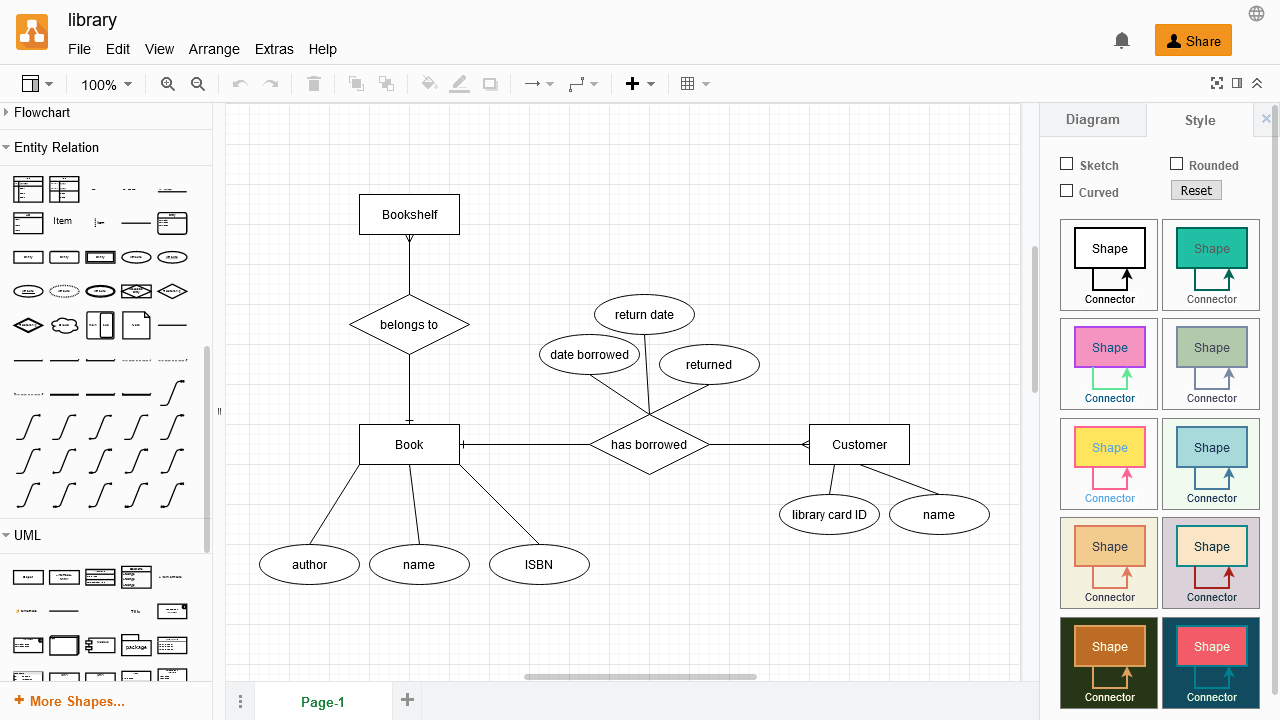
\includegraphics[width = \textwidth]{../img/diagrams.net.png}
  \caption{Tvorba ER diagramu v~aplikaci diagrams.net}
  \label{fig:diagrams.net}
\end{figure}

\section{drawSQL}

Srovnávací kritéria:
\begin{itemize}
  \item kategorie -- logická vrstva,
  \item typ úložiště -- online, poskytované autory produktu
  \item export -- schematický (obecný SQL i~platformě specifické formáty), rastrový \acrshort{png}, serializovaný (JSON~\cite{tc39group_jsondata_2017}, v~době psaní práce se chystá)
  \item interaktivní spolupráce -- pouze v~placené verzi,
  \item komercializace -- omezená verze navždy zdarma, různé měsíčně placené plány.
\end{itemize}

Nástroj drawSQL~\cite{drawsql_2021} je modelovací nástroj pro tvorbu relačních schémat.
Aplikace je dostupná ve webovém prohlížeči\footnote{na adrese \url{https://drawsql.app}}.
Je vyvinuta ve standardních webových technologiích a~používá framework Vue.js.
Plán zdarma umožňuje tvorbu veřejně přístupných diagramů, které mohou mít maximálně 15 tabulek (entit).
Měsíčně placené plány umožňují vytvářet neveřejné diagramy, více (až neomezeně mnoho) tabulek v~diagramu, více uživatelů, kteří mohou na diagramu spolupracovat, a~přístup k~verzovacím nástrojům.
K~vyzkoušení i~používání nástroje je potřeba uživatelský účet.

Hlavní funkcí drawSQL je export schématu do SQL.
Proto si uživatel při vytváření diagramu zvolí cílovou databázi, pro kterou schéma tvoří.
Výsledné SQL tak bude mít tvar, se kterým cílová databáze umí pracovat.
Podporovanými databázemi jsou
MySQL\footnote{\url{https://mysql.com}},
PostgreSQL\footnote{\url{https://postgresql.org}}
a~SQL Server\footnote{Microsoft SQL Server -- \url{https://aka.ms/sqlserver}}.

Rozhraní, které je vidět na Obrázku~\ref{fig:drawsql}, obsahuje diagram a~postranní panel.
V~postranním panelu lze vytvářet jednotlivé tabulky, definovat jejich sloupce a~vlastnosti jednotlivých sloupců -- typ sloupce,
nullability\footnote{\emph{nullability} je příznak, který určuje, zda lze sloupec v~řádku nastavit na hodnotu \texttt{NULL}},
zda se jedná o~primární klíč, unikátní klíč nebo index.
Tyto změny se v~reálném čase reflektují v~diagramu, ve kterém může uživatel jednotlivé sloupce spojovat, čímž vytváří cizí klíče.
Pozici těchto lomených čar lze upravovat pouze posunutím tabulky v~diagramu.
Pokud je cizích klíčů víc, začne být diagram velmi nepřehledný.

Diagram lze importovat ze souboru SQL stisknutím \menu{File > Import}.
Stisknutím tlačítka \menu{File > Export} se otevře nabídka Export, ve které může uživatel diagram exportovat do SQL své předem zvolené databáze, nebo do rastrového obrázku ve formátu \acrshort{png}.
Vývojáři aplikace plánují implementovat také export diagramu pomocí serializace do formátu JSON.
V~nabídce Export je navíc možnost nechat si vygenerovat platformně specifický kód jako například migrační třídy pro
Laravel\footnote{Framework pro PHP -- \url{https://laravel.com}},
definice modelů pro Laravel, a~migrační schémata pro
AdonisJS\footnote{Framework pro Node.js -- \url{https://adonisjs.com}}.

Interaktivní spolupráce je k~dispozici pouze v~placené verzi.
Dle našeho názoru je interaktivní spolupráce hlavní funkcí tohoto nástroje oproti konkurenčním relačním modelovacím nástrojům.
Některá integrovaná vývojová prostředí (např. Visual Studio\footnote{Vývojové prostředí Microsoft Visual Studio -- \url{https://visualstudio.microsoft.com}}) obsahují nástroj pro relační modelování i~generování databázového schématu.
Hlavním omezením těchto nástrojů je však absence interaktivní spolupráce, jedná se spíše o~spolupráci iterací.
Proto považujeme určení interaktivní spolupráce za placenou funkci za negativní rozhodnutí pro využitelnost nástroje v~relaci s~konkurencí.

Web drawSQL také zveřejňuje šablony modelů\footnote{na adrese \url{https://drawsql.app/templates}} (jedná se spíše o~příklady).
Šablony jsou většinou potenciální modely známých produktů (např. WordPress\footnote{\url{https://wordpress.com}}) a~tvoří je autoři drawSQL.
Tuto funkci považujeme za výhodu, protože společnosti a~individuální vývojáři se mohou inspirovat existujícími a~ověřenými řešeními, případně nezačínat se svým modelem od nuly.

Závěrem určíme výhody drawSQL:
\begin{itemize}
  \item příjemné uživatelské rozhraní (viz Obrázek~\ref{fig:drawsql}),
  \item možnost určení typu relace, o~sémantiku se aplikace stará sama (one-to-one, one-to-many, many-to-many),
  \item několik platformě specifických generátorů modelu,
  \item šablony a~příklady existujících modelů
\end{itemize}
a~nevýhody:
\begin{itemize}
  \item nelze upravit ani přesunout lomené čáry spojující cizí klíče, což způsobuje chaos pokud je v~diagramu větší množství entit,
  \item interaktivní spolupráce pouze v~placeném plánu,
  \item správa verzí pouze v~placeném plánu,
  \item k~vyzkoušení nástroje je potřeba uživatelský účet,
  \item podporuje pouze relační databáze.
\end{itemize}

\begin{figure}
  \centering
  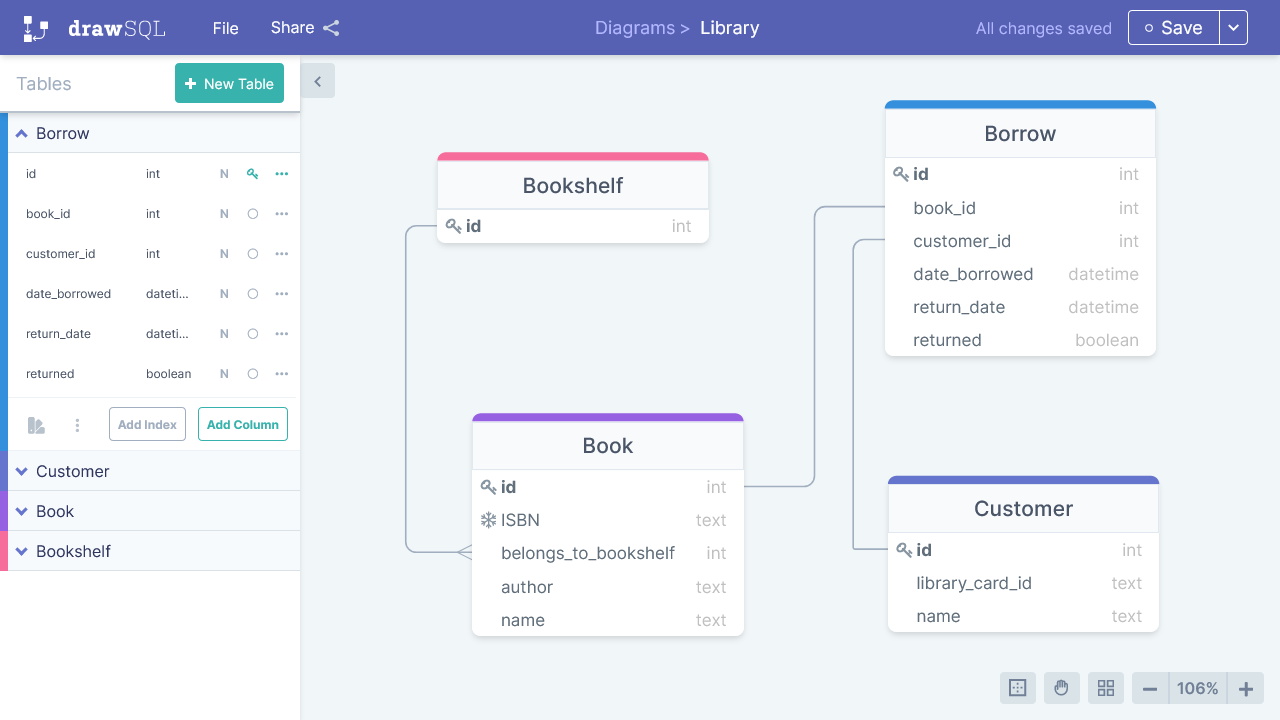
\includegraphics[width = \textwidth]{../img/drawsql.png}
  \caption{Tvorba diagramu v~drawSQL}
  \label{fig:drawsql}
\end{figure}

\section{ERDPlus}
\begin{itemize}
  \item kategorie -- logická vrstva,
  \item typ úložiště -- online, poskytované autory produktu
  \item export -- rastrový \acrshort{png},
  \item interaktivní spolupráce -- není,
  \item komercializace -- zdarma.
\end{itemize}

Nástroj ERDPlus~\cite{erdplus_2023} je modelovací nástroj pro tvorbu ER diagramů, relačních schémat a~hvězdicových schémat.
Aplikace je dostupná ve webovém prohlížeči\footnote{na adrese \url{https://erdplus.com}}.
Její uživatelské rozhraní je tedy vyvinuto ve standardních webových technologiích -- HTML, CSS a~JavaScript.
Dále využívá framework React~\cite{react_2023} pro tvorbu rozhraní v~jazyce JavaScript.

ERDPlus lze používat bez založení uživatelského účtu a~vytvořený diagram exportovat do speciálního formátu erdplus, nicméně uživatel tak přijde o~možnost využití úložiště diagramů na serveru aplikace.
Diagramy (ERDPlus je nazývá \emph{dokumenty}) lze organizovat do složek a podsložek.
Služby ERDPlus včetně úložiště nejsou žádným způsobem zpoplatněny.

Tvorba ER diagramů je intuitivní s~jednoduchým uživatelským rozhraním, které je vidět na Obrázku~\ref{fig:erdplus}.
Uživatel má na výběr mezi vytvořením entity, atributu, relace, spojení mezi těmito objekty a~jednoduchého textového popisku.
V~pravé části rozhraní se nachází panel s~vlastnostmi zvoleného objektu.
V~tomto panelu může uživatel také rychleji tvořit atributy entit a~relací.
Při zvolení relace lze v~panelu zvolit entity, které mají být v~relaci, a~spojení je pak automaticky vytvořeno.
Zároveň lze zvolit jednotlivé multiplicity relace.

Soubor s~diagramem je v~úložišti reprezentován vlastním formátem erdplus.
Jedná se o~textový soubor, jehož obsahem je JSON reprezentace diagramu.
Diagram lze exportovat do rastrového formátu \acrshort{png}.

Zajímavou funkcí je také převod do relačního schématu.
Tato funkce je dostupná pouze tehdy, když uživatel ER diagram uloží na server ERDPlus.
Poté zvolí možnost \emph{Convert to Relational Schema} a~ERDPlus vytvoří nové relační schéma.
Z~relačních schémat lze podobně vygenerovat SQL.

Vlastnoruční tvorba relačních diagramů probíhá podobně.
Uživatel může tvořit tabulky, přidávat jim sloupce a v~tabulkách volit primární klíče v~postranním panelu.
Pomocí tlačítka \texttt{Connect} lze poté přidat cizí klíč, který odkazuje do jiné tabulky tažením myši.
ERDPlus do tabulky přidá všechny primární klíče, které cílová tabulka obsahuje, jako nové sloupce.
K~vytvoření cizího klíče, který odkazuje na stejnou tabulku (tzv. rekurzivní klíč) slouží tlačítko \texttt{Recursive Key} ve vlastnostech tabulky.
Hvězdicovým schématům se věnovat nebudeme, protože jsou mimo rozsah této práce.

Výhody:
\begin{itemize}
  \item převod diagramu z~ER do relačního diagramu,
  \item jednoduchost a intuitivnost procesu kresby diagramu
\end{itemize}
a nevýhody:
\begin{itemize}
  \item relační diagram bývá nepřehledný, nelze měnit pořadí jednotlivých definovaných sloupců v~tabulce,
  \item chybí vektorový export,
  \item diagramy nelze stylizovat.
\end{itemize}

\begin{figure}
  \centering
  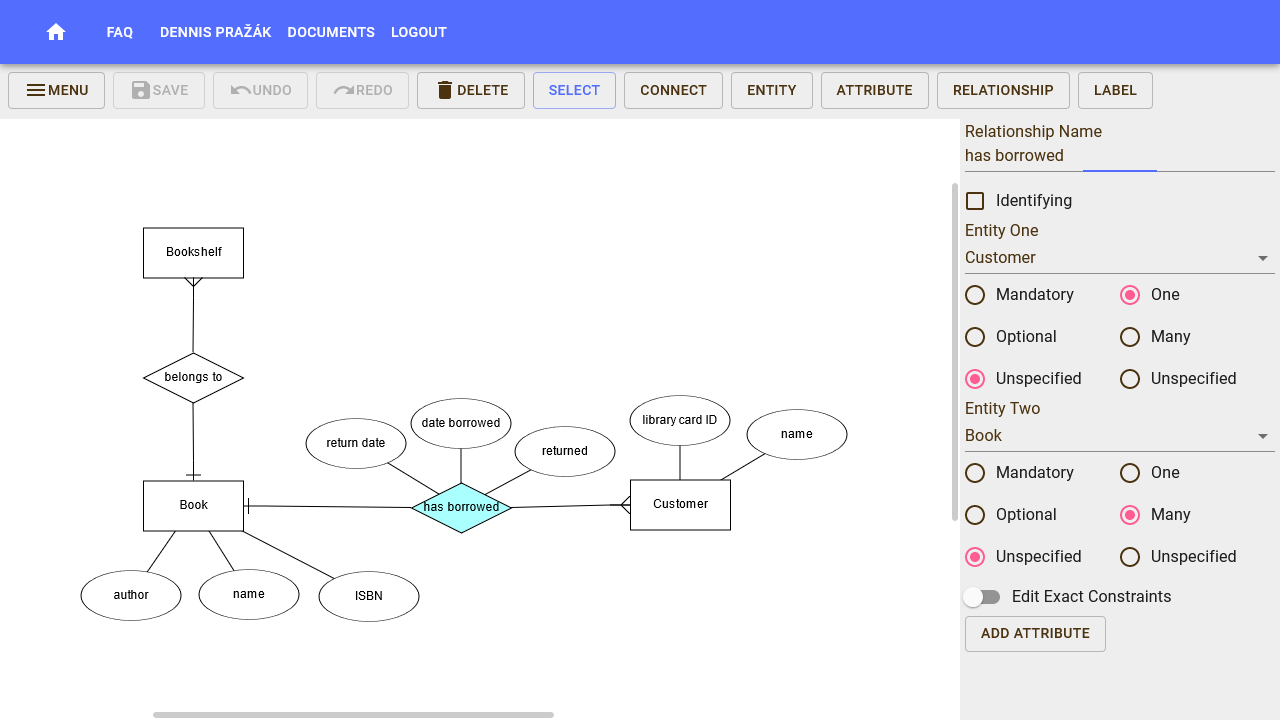
\includegraphics[width = \textwidth]{../img/erdplus.png}
  \caption{Tvorba ER diagramu v~ERDplus}
  \label{fig:erdplus}
\end{figure}

\section{nomnoml}

\begin{itemize}
  \item kategorie -- kresba omezených diagramů -- UML,
  \item typ úložiště -- online,
  \item export -- rastrový \acrshort{png}, vektorový \acrshort{svg},
  \item interaktivní spolupráce -- není k~dispozici,
  \item komercializace -- zdarma s~otevřeným zdrojovým kódem.
\end{itemize}

Nástroj nomnoml je modelovací nástroj pro tvorbu UML diagramů dostupný ve webovém prohlížeči\footnote{na adrese \url{https://nomnoml.com}}.
Jeho klíčová vlastnost je, že místo interakce myší s~webovou aplikací probíhá kresba deklarativně -- psaním.

Uživatelské rozhraní (viz Obrázek~\ref{fig:nomnoml}) se skládá z~oblasti pro textový vstup, nad kterou je zároveň (v~reálném čase) vykreslován výsledný diagram.
V~pravé horní části se nachází několik tlačítek, při kliknutí na některé z~nich se vždy otevře pravý postranní panel s~odpovídajícími informacemi a funkcemi.
První tlačítko ukazuje rychlý přehled jazyka, ve kterém se má diagram definovat.
Druhé tlačítko odhalí kompletní referenci k~tomuto jazyku.
Dále lze najít tlačítka pro export, sdílení a uložení do místního úložiště uživatele.

Jazyk diagramů je velmi jednoduchý.
Skládá se z~definic entit a jejich relací.
Uživatel může vyjít z~úvodního diagramu, který se ukáže při navštívení hlavní stránky nástroje.
Pro ukázku, definice entity vypadá následovně

\noindent\texttt{[<abstract> Entita|soukromaSlozka; soukromaSlozka2|verejnyAtribut]}.

Svislá čára odděluje kategorie atributů, může jich být neomezené množství.
Entita je definována jako abstraktní, což také ovlivní její výsledný styl vzhledu v~diagramu.

Dále se v~jazyce definují vztahy mezi entitami \texttt{[Entita]->[Entita2]}.
Různé šipky mají různé významy.
Vztah \texttt{->} je \emph{asociace}, dále \texttt{o->} je \emph{agregace}, apod.

V~jazyce lze také deklarovat direktivy, začínající znakem \texttt{\#}.
Těmi může uživatel upravit vzhled, vytvořit nové styly, a nastavit algoritmy, kterými bude zvoleno rozložení entit v~diagramu.
Algoritmy lze nastavit direktivou \texttt{\#ranker} a na výběr je ze tří možností: \texttt{network-simplex}, \texttt{tight-tree}, \texttt{longest-path}.
Nástroj nomnoml používá k~vykreslování diagramu knihovnu dagre\footnote{\url{https://github.com/dagrejs/dagre}} pro JavaScript, jejíž vývoj byl však ukončen.
Z~dokumentace této knihovny vyplývá, že možnost \emph{ranker} mění algoritmus, který vrcholům v~grafu (diagramu) přiřazuje důležitost, která se pak odráží v~pořadí zobrazení entit.
Definitivní význam této možnosti není z~dokumentace zřejmý, u~nástroje nomnoml lze však pozorovat změnu v~pořadí a vzdálenostech entit (délce spojovacích čar).
Uživatel tak může vyzkoušet různá rozložení a použít to, které je vizuálně nejpřehlednější.

Diagram lze exportovat do formátu \acrshort{png} a dále podobně jako v~sekci~\ref{section:drawio}, nomnoml také umožňuje export do \acrshort{svg} se zakomponovaným zdrojovým kódem.
Uživatel tak může diagram distribuovat v~tomto formátu a zároveň tento formát v~nástroji nomnoml i otevřít a plnohodnotně pokračovat v~práci.
Podobně je možné sdílet odkaz přímo na vytvořený diagram ve službě nomnoml.
Odkaz je vytvořen tak, že do URL je jako parametr \texttt{source} zapsán přímo zdrojový kód diagramu.
Výsledná adresa URL je tak velice dlouhá, ale služba nomnoml nemusí diagramy ukládat, stačí je vykreslit z~dat v~odkazu.
Přestože se nejedná o~opravdové online úložiště, kategorizovali jsme ho tímto způsobem.
Rozdělaný diagram lze také uložit do paměti prohlížeče.
Díky těmto mechanismům stačí službě nomnoml staticky poskytovat pouze klientskou stranu své aplikace a přesto umožňuje ukládání a sdílení práce.

Nástroj nomnoml je tedy inovativní svým přístupem ke kresbě diagramů.
U~složitých diagramů se však nutně ve zdrojovém kódu uživatel ztrácí, protože nomnoml nenabízí žádné dělení či kompozici tohoto kódu.
S~vizuální reprezentací grafu nelze přímo (např. myší) pracovat, veškeré rozložení a orientaci diagramu tak musí uživatel nechat na algoritmu nástroje.
Nástroj dále nenabízí ani možnost pracovat s~několika diagramy najednou.
Z~těchto důvodů určujeme produkt jako vhodný pouze pro jednotlivce a tvorbu méně rozsáhlých UML diagramů.

\begin{figure}
  \centering
  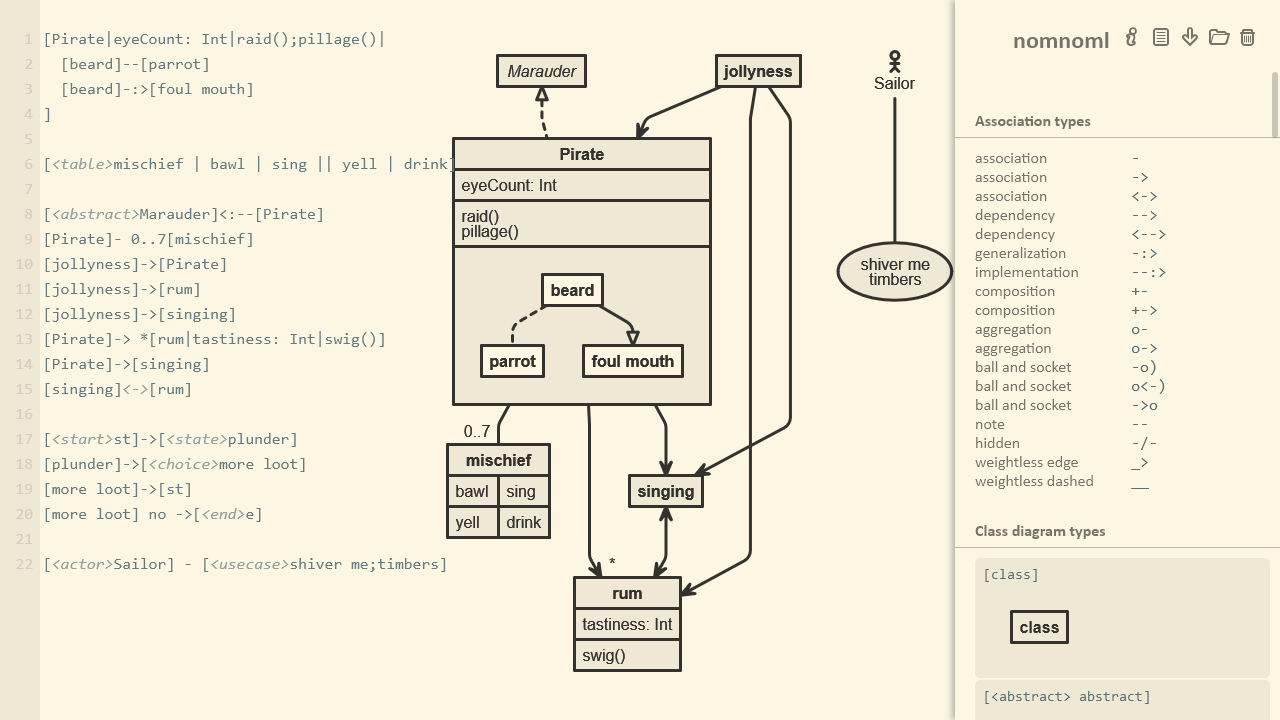
\includegraphics[width = \textwidth]{../img/nomnoml.png}
  \caption{Tvorba UML diagramu v~nomnoml}
  \label{fig:nomnoml}
\end{figure}

\section{Visual Paradigm Online}

Srovnávací kritéria:
\begin{itemize}
  \item kategorie -- kresba libovolných diagramů,
  \item typ úložiště -- online, lokální, externí, prohlížeč,
  \item export -- serializovaný, rastrový, vektorový,
  \item interaktivní spolupráce -- podporována,
  \item komercializace -- verze zdarma, měsíčně/ročně placené plány několika úro\-vní.
\end{itemize}

Nástroj Visual Paradigm Online\footnote{\url{https://online.visual-paradigm.com}} je proprietární produkt od firmy Visual Paradigm.
Tato firma je známá svou stejnojmennou desktopovou aplikací, která má stejný účel. Zde se zaměříme na její online verzi.

Visual Paradigm Online je nástroj pro tvorbu různých typů diagramů.
Mimo těch je určen i pro úpravu fotografií, tvorbu koláží, design infografiky, příspěvků na sociální sítě, uživatelských rozhraní, plakátů, dárkových poukazů, apod.
Funkcionalita kromě tvorby diagramů je mimo rozsah této práce.

Nástroj poskytuje předlohy tvarů pro diagramy tříd, use case diagramy, sekvenční diagramy, diagramy aktivit, diagramy nasazení (deployment), ER diagramy a velmi mnoho dalších.
Uživatel si před tvorbou diagramu musí vybrat jednu z~těchto kategorií, čímž vymezí tvary, které jsou v~uživatelském rozhraní dostupné k~použití v~levém postranním panelu.
Ve stejném panelu lze ale posléze přidat libovolnou další kategorii tvarů dle výběru uživatele.

Nástroj je svým rozhraním, designem a chováním nápadně podobný produktu diagrams.net ze sekce~\ref{section:drawio}.
Stejně tak spojování tvarů čarami má velmi podobné chování.
Jeden rozdíl je ten, že kresba spojení z~jednoho tvaru do toho samého (tvorba "cyklu") je velmi nepředvídatelná.
Čára se při tom samovolně přemisťuje do všech možných stran, až nakonec zůstane přilepena na jedné ze stran tvaru.

Diagramy lze uložit do formátu \texttt{vpd}, který při otevření v~textovém editoru připomíná base64 kód.
Vypadá velice podobně jako serializace pro diagrams.net ze sekce~\ref{section:drawio}.
Nejedná se však o~validní base64 kód, protože ten kóduje 3 bajty do 4 znaků, jinak používá výplň 0-2 znaky \texttt{=}.
Nicméně \texttt{vpd} obsahuje i sekvence jako je \texttt{M=Q8}, které tomu neodpovídají.
Jedná se tak nejspíš o~nezdokumentovaný proprietární formát.

Diagramy lze exportovat do formátu \acrshort{svg} a PDF, do kterých lze volitelně uložit i serializaci diagramu ve formátu \texttt{vpd} a případně tak plnohodnotně přenést editovatelný diagram i s~jeho vektorovou reprezentací.
Rastrový export je možný ve formátu JPEG nebo \acrshort{png}.
Stejně jako u~diagrams.net ze sekce~\ref{section:drawio} je do \acrshort{png} volitelně přidána serializace diagramu v~\texttt{tEXt} chunku formátu \acrshort{png}.
Dokonce je použito stejné klíčové slovo identifikující tuto serializaci -- \texttt{mxfile}.
To vzbuzuje podezření, že se jedná o~stejný formát, jako používá diagrams.net ze sekce \ref{section:drawio}, tedy formát serializace modelu diagramu knihovny mxGraph\footnote{\url{https://jgraph.github.io/mxgraph/}}.
O~tom, že Visual Paradigm Online používá stejný formát jsme ale nenašli žádné zmínky.
Dále, jak už bylo zmíněno, \texttt{vpd} nemá stejnou strukturu jako mxfile\footnote{\url{https://drawio-app.com/extracting-the-xml-from-mxfiles/}}.

Komercializace Visual Paradigm Online je rozdělena do několik platebních úrovní.
Každá úroveň má určenou cenu za uživatele za měsíc.
Úrovně jsou dle ceny a úplnosti funkcí vzestupně Free (zdarma), Starter, Advance, Combo (všechny funkce).
Úroveň Free obsahuje i prémiové šablony, ale je v~nich zobrazen vodoznak.
Ten je v~placených plánech odstraněn.
Placené plány navíc obsahují více typů diagramů a více tvarů k~použití, rastrový export vyššího rozlišení, historii verzí diagramu (při spolupráci) a další.

\section{Závěr existujících řešení}

Přehled analýzy zmíněných existujících řešení je vidět v~Tabulce~\ref{tab:existing-comparison}.

\newcommand{\tnote}[1]{\textsuperscript{#1}}
\begin{table}
  \begin{center}
    \sffamily
    \tabcolsep = 1pt\relax
    \footnotesize
    \makebox[\textwidth]{
      \begin{tabular}{r|c|c|c|c}
        \toprule
        název produktu     & \textbf{diagrams.net}                   & \textbf{drawSQL}                 & \textbf{ERDPlus} & \textbf{nomnoml}                   \\
        \midrule
        kategorie (vrstva) & libovolné d.                            & logická                          & konceptuální     & omezené d.                         \\
        serializovaný ex.  & ano                                     & ne\tnote{\ref{tab:ec:plan}}      & ano              & ano                                \\
        rastrový ex.       & ano                                     & ano                              & ano              & ano                                \\
        vektorový ex.      & ano                                     & ne                               & ne               & ano                                \\
        schematický ex.    & ne                                      & SQL                              & SQL              & ne                                 \\
        zjednodušený ex.   & HTML, PDF                               & ano\tnote{\ref{tab:scaffolding}} & ne               & ne                                 \\
        poskytuje úložiště & ne\tnote{\ref{tab:ec:external-storage}} & ano                              & ano              & ano\tnote{\ref{tab:ec:urlsharing}} \\
        paměť prohlížeče   & ano                                     & ne                               & ne               & ano                                \\
        \midrule[\heavyrulewidth]
      \end{tabular}
    }
  \end{center}

  \footnotesize
  \begin{enumerate}[a.,ref = \alph*,noitemsep]
    \item plánovaná funkce \label{tab:ec:plan}
    \item využívá úložiště třetích stran \label{tab:ec:external-storage}
    \item platformně-specifický scaffolding -- automatické generování kódu pro specifické platformy a programovací jazyky \label{tab:scaffolding}
    \item diagram je uložen v~URL, pomocí které lze diagram sdílet \label{tab:ec:urlsharing}
  \end{enumerate}

  \caption{Srovnání existujících řešení}
  \label{tab:existing-comparison}
\end{table}

\chapter{Specifikace}

Sommerville~\cite{sommerville_software_2011} % strana 6
uvádí fundamentální aktivity softwarového inženýrství: specifikace, vývoj, validace a evoluce.
Dále definuje softwarovou specifikaci jako aktivitu, při které zákazníci a inženýři definují software, který má být vyprodukován, a omezení na jeho provoz. % strana 9

V této kapitole definujeme software, který budeme tvořit, pomocí požadavků uživatele, případů užití, diagramu tříd v konceptuální vrstvě a procesů.

\section{Požadavky}

Požadavky na softwarový systém jsou popisy toho, co by měl systém dělat -- služby, které poskytuje, a omezení na jeho provoz.
Tyto požadavky by měly reflektovat potřeby zákazníka na systém a jeho účel, uvádí Sommerville~\cite[s.~83]{sommerville_software_2011}. % strana 83

Požadavky na funkce systému nazýváme funkční.
Požadavky na provoz systému a jeho omezení nazýváme nefunkční.

Dále uvedeme vybrané funkční a nefunkční požadavky z pohledu uživatele systému.

\subsection{Funkční požadavky}
\newlist{enumfp}{enumerate}{1}
\setlist[enumfp]{label=\textbf{FP-\arabic*},ref=FP-\arabic*}

\subsubsection*{Projekt}

\begin{enumfp}
    \item V systému bude možné vytvořit nový projekt.
    \item Projekt bude možné uložit.
    \item Projekt bude možné načíst.
    \item Jednotlivé diagramy bude možné exportovat do rastrového i vektorového obrázku.
\end{enumfp}

\subsubsection*{ER Diagram}

\begin{enumfp}[resume]
    \item 
\end{enumfp}

\subsection{Nefunkční požadavky}
\newlist{enumnfp}{enumerate}{1}
\setlist[enumnfp]{label=\textbf{NFP-\arabic*},ref=NFP-\arabic*}

\begin{enumnfp}
    \item Aplikaci bude možné používat na všech běžných desktopových operačních systémech.
    \item Nesmí dojít ke ztrátě práce při pádu aplikace kvůli interním či externím vlivům.
    \item Aplikaci bude možné používat bez internetového připojení.
\end{enumnfp}

% \chapter{Specifikace}\label{chapter:specifikace}

V této kapitole navrhneme software, který plánujeme implementovat, pomocí požadavků, konceptuálního datového modelu, procesů, tříd a scénářů.
Kromě toho také uvedeme koncept řešení, který poskytne rychlý přehled toho, jak bude systém technologicky navržen.
Řídíme se tak běžným postupem softwarového inženýrství~\cite{sommerville_softwareengineering_2011}.

\section{Požadavky}

V této sekci představíme funkční a nefunkční požadavky na systém~\cite[s.~83]{sommerville_softwareengineering_2011}.

\subsection{Funkční požadavky}
Vzhledem k většímu množství funkčních požadavků je rozdělíme do několika kategorií, které budou seskupovat požadavky týkající se podobné části systému.

\subsubsection*{Projekt}
\begin{itemize}
  \item Součástí projektu budou tři typy diagramů -- \acrshort{er}, schematická kategorie a vizualizace schematické kategorie.
  \item Projekt bude obsahovat data, z kterých bude možné obnovit všechny tři diagramy, na kterých uživatel pracuje během jednoho sezení.
  \item V systému bude možné vytvořit nový projekt, uložit ho a načíst.
  \item Projekt bude možné pojmenovat pro odlišení od ostatních projektů.
\end{itemize}

\subsubsection*{Export}
\begin{itemize}
  \item Jednotlivé diagramy bude možné exportovat do rastrového i vektorového formátu.
  \item Do těchto exportovaných formátů bude volitelně možné vložit projekt, který z nich pak bude možné načíst.
        Tímto bude projekt možné otevřít jak v prohlížeči obrázků (a zobrazit rastrově nebo vektorově diagram), tak v našem systému a pokračovat v práci.
  \item Při exportu do \acrshort{png} bude možný výběr mezi průhledným a celobarevným pozadím.
\end{itemize}

\subsubsection*{Diagramy}
\begin{itemize}
  \item Zobrazení diagramu bude možné posouvat myší.
  \item Zobrazení diagramu bude možné přibližovat a oddalovat kolečkem myši.
  \item Posunutí a přiblížení bude volitelně možné synchronizovat mezi všemi diagramy.
  \item Systém bude kontrolovat validitu uživatelem vytvořených konstruktů.
  \item Elementy bude možné posunovat držením levého tlačítka myši a tažením.
  \item Související elementy napříč diagramy se volitelně budou posouvat společně.
  \item Vlastnosti všech objektů bude možné měnit (popisky, typ, pozice).
        Tyto změny budou reflektovány v ostatních diagramech.
  \item Při držení klávesy \keys{\ctrl} bude možné zvolit více objektů najednou postupným klikáním levého tlačítka myši.
  \item Veškeré elementy bude možné z diagramu mazat alespoň klávesou \keys{Delete}.
  \item Všechny elementy bude možné zvolit levým tlačítkem myši.
\end{itemize}

\subsubsection*{ER Diagram}
\begin{itemize}
  \item Do diagramu bude možné přidat entitní typ (silné i slabé), vztahový typ, atribut (včetně složeného atributu),
  \item K entitním typům bude možné přidat identifikátory, včetně externích.
  \item Bude možné vytvořit ISA hierarchii mezi entitními typy.
  \item Mezi jednotlivými elementy diagramu bude možné přidat spojovací čáru.
  \item U spojení bude možné specifikovat a zobrazit kardinalitu.
        Dolní mez bude buď 0 nebo 1, horní mez 1 nebo $n$.
        Výchozí kardinality \oneone{} nebudou zobrazeny.
  \item Uživatel bude moct využít předpřipravené konstrukty, které bude možné vložit do diagramu.
        Například se může jednat o ISA hierarchie s předpřipravenými entitami.
\end{itemize}

\subsubsection*{Schematická kategorie}
\begin{itemize}
  \item Objekty a morfismy schematické kategorie bude možné přidávat a mazat, přičemž tato změna se odrazí v ostatních diagramech.
  \item V diagramu se zobrazí data o objektech a morfismech včetně kardinalit a popisků.
        Výchozí kardinality \oneone{} se zobrazovat nebudou.
  \item Při zvolení objektu se zvýrazní všechny objekty v okolí, které ho identifikují (např. barevně, vzdálené identifikátory jinou barvou).
\end{itemize}

\subsubsection*{Vizualizace schematické kategorie}
\begin{itemize}
  \item Vizualizace schematické kategorie ze schematické kategorie zjistí sémantiku a vizualizuje ji různými tvary.
  \item Objekty a morfismy bude možné přidávat a mazat i ve vizualizaci schematické kategorie.
  \item Při zvolení objektu se barevně zvýrazní bezprostřední a vzdálené identifikátory různými barvami.
\end{itemize}

\subsection{Nefunkční požadavky}

\begin{itemize}
  \item Aplikaci bude možné používat na všech běžných desktopových operačních systémech.
  \item Nesmí dojít ke ztrátě práce při náhlém ukončení aplikace kvůli interním či externím vlivům.
        To může být zařízeno např. průběžným ukládáním práce.
  \item Aplikaci bude možné používat i při výpadku internetového připojení.
  \item V rámci bezpečnosti žádná data týkající se práce na projektu neopustí zařízení klienta, pokud tak klient explicitně neučiní (například export a přesun souboru).
  \item Aplikace bude navržena tak, aby bylo možné bez větších komplikací rozšířit její funkcionalitu (např. přidat podporu UML).
  \item Aplikace bude nenáročná na provoz a investice provozovatele.
\end{itemize}

\section{Entity}\label{section:conceptual-model}

V této kapitole představíme konceptuální datový model aplikace.
Využijeme k tomu prostředky \acrfull{uml}~\cite{omg_uml_2017}.

\begin{figure}[!htb]
  \centering
  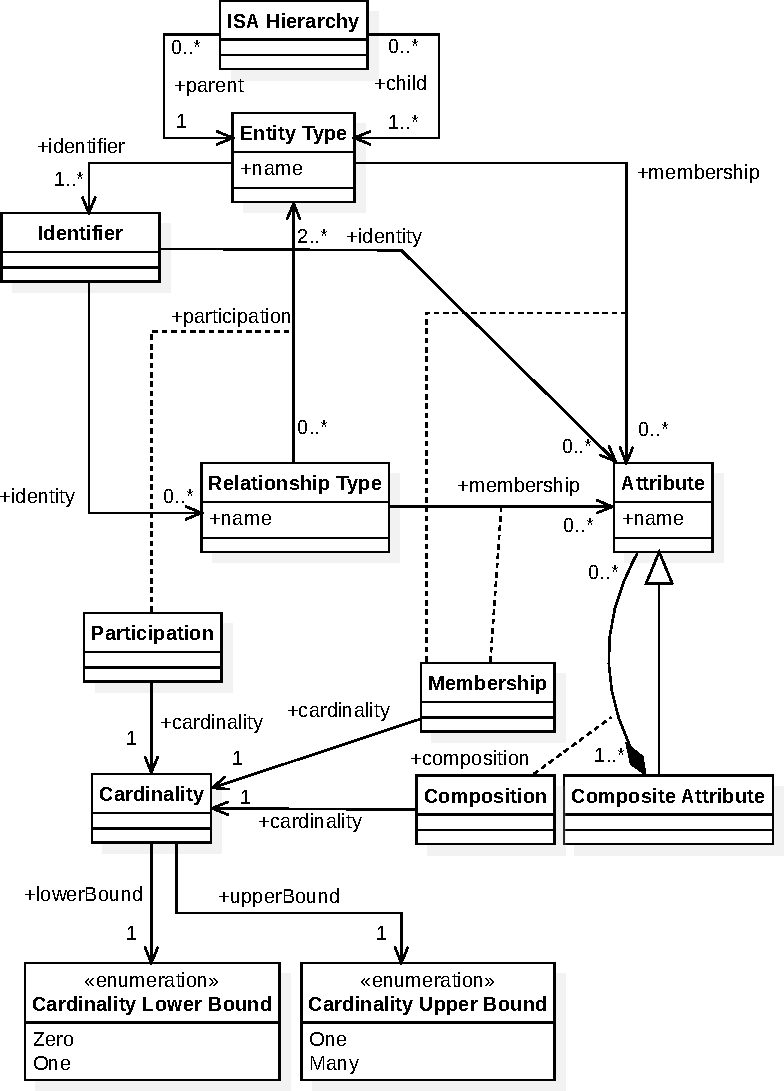
\includegraphics[width=\maxwidth{\textwidth}]{../img/diagrams/er-diagram-model.pdf}
  \caption{Konceptuální schéma -- ER diagram}
  \label{fig:class-diagram:er-diagram}
\end{figure}

Na Obrázku~\ref{fig:class-diagram:er-diagram} je \acrshort{UML} konceptuální schéma modelující \acrshort{er} diagram.
Obsahuje třídy odpovídající všem konstruktům popsaných v Sekci~\ref{section:entity-relationship} -- entitní typ, vztahový typ, atribut, složený atribut, ISA hierarchie, kardinalita a identifikátor.
Entitní typ, vztahový typ i atribut mají složku vyjadřující jejich uživatelské jméno.
Navíc jsme uvedli tři třídy asociace k asociacím mezi těmito objekty, které mají všechny svou kardinalitu:
\begin{itemize}
  \item \emph{Membership} (členství) vyjadřuje vztah mezi entitním typem nebo vztahovým typem a atributem.
        Toto jméno vyjadřuje, že atributy považujeme za členy (members) entitních a vztahových typů.
        Entitní i vztahové typy mají buď žádný atribut, nebo libovolné množství atributů.
  \item \emph{Composition} (složení) vyjadřuje vztah mezi složeným atributem a atributy, z kterých se skládá.
        Složený atribut musí mít alespoň jeden atribut, jinak ho nepovažujeme za složený.
  \item \emph{Participation} (účast) vyjadřuje vztah mezi vztahovým typem a entitními typy, které se daného vztahového typu účastní.
\end{itemize}

Názvy pro naše tři třídy asociace byly inspirovány \acrshort{er} diagramem, který modeluje \acrshort{er} od Atzeniho~\cite[Obr.~5.22]{atzeni_database_1999}

Tyto tři třídy asociace jsme mohli sjednotit do jedné, protože všechny obsahují pouze jednu instanci kardinality.
Tím by však zanikl jejich rozlišný význam, který může být v určitém kontextu důležitý.
Mohli bychom jim také uvést společného předka, ale to považujeme za zbytečné a konceptuálně nemnoho vypovídající.

Kardinalita se skládá ze dvou složek, jejichž možné hodnoty jsou dány enumeracemi.
To vyjadřuje naše omezení, která jsme na kardinalitu položili.

ISA hierarchie se přesně podle definice skládá z jednoho entitního typu rodiče a jednoho či více entitních typů dětí.
Mohli jsme místo toho modelovat vztah jednoho rodiče s jedním dítětem, ale v \acrshort{er} je důležité nad těmito vztahy uvažovat po $n$-ticích.

Identifikátory jsme namodelovali bez rozlišení významu externích a interních identifikátorů, protože to je vlastnost, která pro každý identifikátor vyplyne až v instanci modelu.
Každý entitní typ musí mít z definice našeho \acrshort{er} modelu alespoň jeden identifikátor.
Ten se může skládat z libovolného množství atributů a vztahových typů.
V instanci modelu bychom označili identifikátor mající alespoň jeden vztahový typ jako externí, jinak interní.
Přestože model technicky povoluje i identifikátory bez členů, nejsou takové identifikátory validní.

\begin{figure}[!htb]
  \centering
  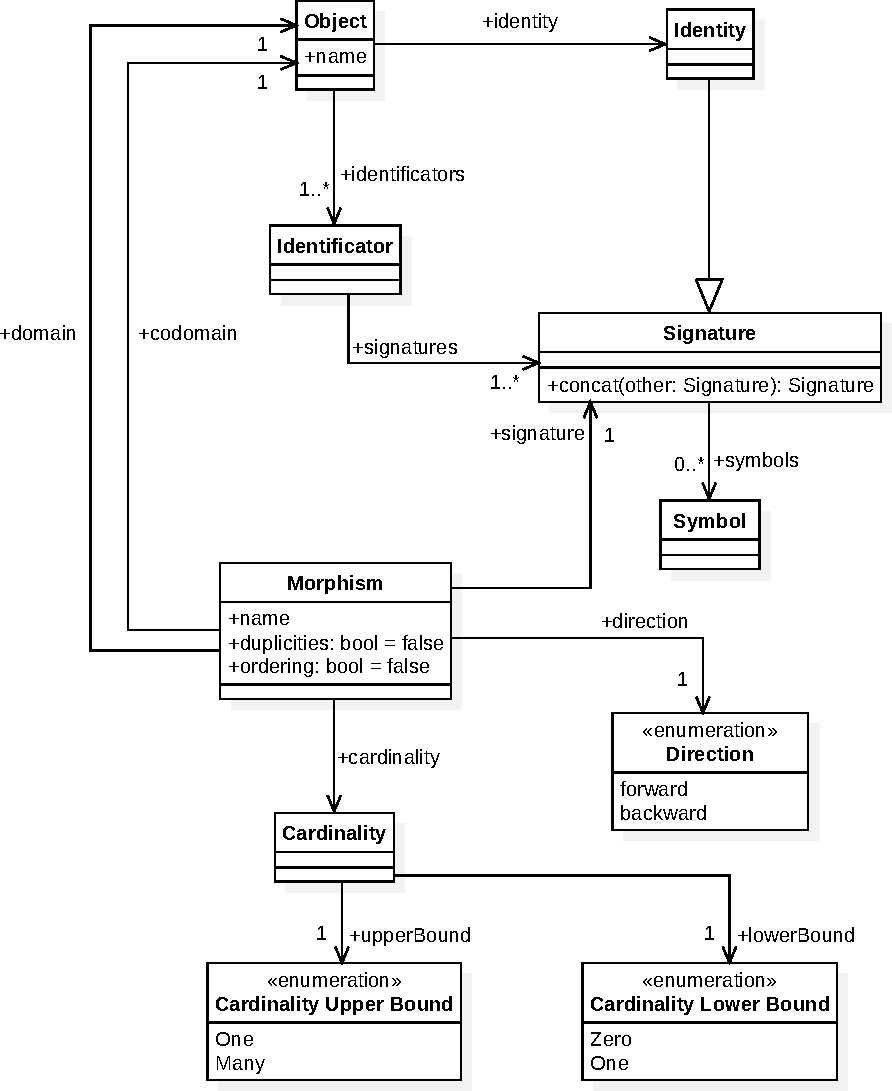
\includegraphics[width=\maxwidth{\textwidth}]{../img/diagrams/schema-category-model.pdf}
  \caption{Konceptuální schéma -- schematická kategorie}
  \label{fig:class-diagram:schemcat}
\end{figure}

Na Obrázku~\ref{fig:class-diagram:schemcat} je konceptuální model schematické kategorie.
Stěžejními třídami v modelu jsou objekt, morfismus a signatura.

Signatura se skládá z jednotlivých symbolů, kterých může být 0 (prázdný řetězec $\varepsilon$) a více.
Jedná se totiž z definice o řetězec.
Jednotlivými symboly budou přirozená čísla.
Signatury půjde navíc řetězit za sebe.
Pokud označíme danou instanci signatury \texttt{tato}, zřetězení by mělo probíhat v pořadí \texttt{tato} $\cdot$ \texttt{další}, stejně jako je to běžné u jazyků.
V implementaci by se mělo dbát na správné pořadí při skládání morfismů, které je opačné a odpovídá pořadí skládání funkcí.

V konceptuálním modelu vyjadřujeme, že každý objekt musí mít alespoň jeden identifikátor, který se skládá ze signatur.
Speciálně tímto identifikátorem může být i $\set{\varepsilon}$, protože signatura může být prázdný řetězec.
Jak jednotlivé identifikátory, tak celá jejich sada u daného objektu, by měla být množina, a proto se nemusí dbát na absenci pořadí a nemožnost duplicit.

Pro morfismy je vyjádřeno, že by měl mít každý svou signaturu.
Mohli bychom morfismy vydělit na námi definované druhy specializováním třídy morfismu na \hlcomment{bázový}{jakto, že odvozených může být nekonečno?}, odvozený a identitní.
U bázových by bylo vyjádřeno, že jejich signaturou je pouze jediný symbol.
U odvozených je jejich signaturou již namodelovaná třída signatury.
A u identitních je jejich signaturou prázdný řetězec, tedy konstanta.
Toto rozdělení nám však pro konceptuální model přijde zbytečné, protože se jedná o vlastnost morfismu, která vyplyne z toho, z kolika symbolů se jeho signatura skládá.

Další prvky konceptuálního modelu schematické kategorie jsou zřejmé a vycházejí přímo z definice schematické kategorie ze Sekce~\ref{section:schemcat}.

\begin{figure}[!htb]
  \centering
  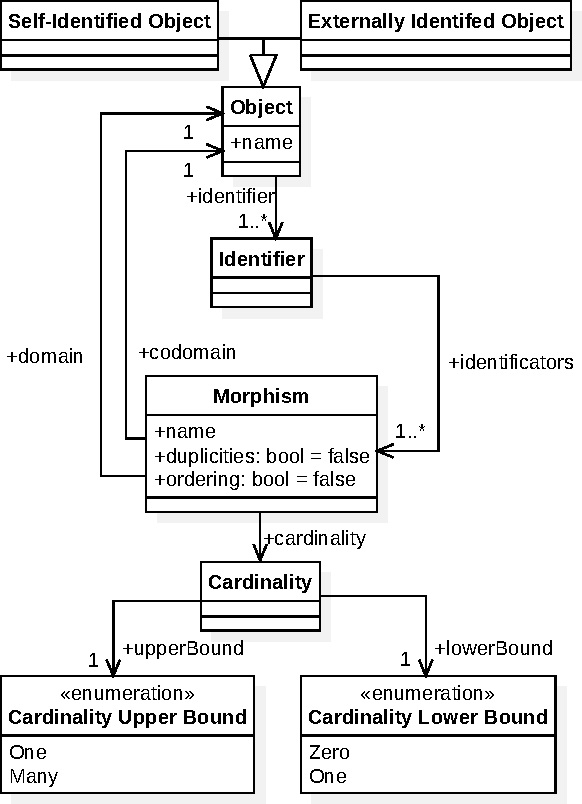
\includegraphics[width=\maxwidth{\textwidth}]{../img/diagrams/scv-model.pdf}
  \caption{Konceptuální schéma -- \acrlong{vsk}}
  \label{fig:class-diagram:scv}
\end{figure}

Konceptuální model vizualizace schematické kategorie, který je na Obrázku~\ref{fig:class-diagram:scv}, je podobný konceptuálnímu modelu schematické kategorie, s několika málo rozdíly.
Duální bázové morfismy splývají do jedné neorientované hrany \texttt{Connection}.
Doména a kodoména původních duálních morfismů se stávají zdrojovým a cílovým objektem daného spojení.
Kvůli tomuto splynutí má také každá výsledná hrana dvě kardinality -- jednu pro každý morfismus, respektive pro každý objekt, který hrana spojuje.
Koncept signatury ve vizualizaci zaniká.
Místo toho jsou identifikátory objektů tvořeny přímo navazujícími morfismy.
Objekty a morfismy ztrácí svoji identitu, resp. signaturu.
Ta konceptuálně ve vizualizaci schematické kategorie není.

V konceptuálním modelu vizualizace schematické kategorie nově rozlišujeme dva typy objektů -- self-identifikovaný objekt (definovaný v Sekci~\ref{section:vsk}) a naproti tomu externě identifikovaný objekt.
Rozlišujeme je kvůli tomu, že ve vizualizaci schematické kategorie jsou tyto odlišné typy objektů zobrazeny různými tvary.

Další koncepty jsou totožné s konceptuálním modelem schematické kategorie.

\section{Procesy}

Součástí specifikace softwarového systému jsou i procesy.
Ty uvedeme v této sekci.

\subsubsection*{Modelování entitního typu v \acrshort{er} diagramu}

Uživatel mezi existující elementy diagramu vloží nový entitní typ.

\noindent Kroky zahrnují:
\begin{enumerate}
  \item Přidání nového prvku do diagramu.
  \item Zvolení druhu prvku -- entitní typ.
  \item Zadání popisku (názvu entitního typu).
  \item Případná změna pozice entitního typu v diagramu.
  \item Případné přidání atributů k entitnímu typu a volba jejich kardinality.
\end{enumerate}

\subsubsection*{Modelování vztahového typu v \acrshort{er} diagramu}
Uživatel bude dále chtít do \acrshort{er} diagramu přidat vztahový typ.
Vztahový typ musí mít alespoň dva (ne nutně různé) účastníky, jimiž mohou být pouze entitní typy.

\noindent Kroky zahrnují:
\begin{enumerate}
  \item Přidání nového prvku do diagramu.
  \item Zvolení druhu prvku -- vztahový typ.
  \item Zadání popisku (názvu vztahového typu).
  \item Zvolení pozice vztahového typu v diagramu.
  \item Zvolení účastníků vztahového typu.
  \item Zvolení kardinalit účastníků vztahového typu.
\end{enumerate}

\subsubsection*{Modelování atributu \acrshort{er} diagramu}
Modelování samostatného atributu může probíhat podobně jako v předchozích scénářích, ale protože se jedná o jeden z nejčastějších procesů, nabídneme alternativně zkratku, kterou zde popíšeme.

\noindent Kroky zahrnují:
\begin{enumerate}
  \item Zvolení entitního nebo vztahového typu, ke kterému přidat atribut, nebo případně zvolení atributu, který se má tímto stát složeným.
  \item Přidání atributu a jeho spojení se zvoleným typem.
  \item Zadání názvu atributu.
  \item Případná změna pozice atributu v diagramu.
\end{enumerate}

\subsubsection*{Editace existujících prvků \acrshort{er} diagramu}
Úprava existujících prvků probíhá pro všechny prvky podobně.
Při modelování může uživatel přehodnotit model a upravit vlastnosti některých prvků.

\noindent Kroky zahrnují:
\begin{enumerate}
  \item Zvolení prvku v diagramu k editaci.
  \item Zvolení vlastnosti prvku, která bude upravena.
  \item Zadání/změna hodnoty vlastnosti prvku.
\end{enumerate}

\subsubsection*{Mazání prvků v \acrshort{er} diagramu}

Při modelování může uživatel přehodnotit model a odstranit některé prvky, načež je případně nahradit jinými.

\noindent Kroky zahrnují:
\begin{enumerate}
  \item Zvolení prvku či prvků v diagramu, které chceme smazat.
  \item Odstranění prvků z diagramu.
  \item Odstranění souvisejících spojení s jinými prvky diagramu.
  \item U entitních typů odstranění případných identifikátorů z diagramu.
\end{enumerate}

\subsubsection*{Volba identifikátoru entitního typu v \acrshort{er} diagramu}

Při modelování entitního typu bude uživatel muset přidat jeho identifikátory.

\noindent Kroky zahrnují:
\begin{enumerate}
  \item Zvolení jednoho a více atributů či vztahových typů, které mají tvořit nový identifikátor.
  \item Přidání identifikátoru do diagramu.
  \item Kontrola validity \acrshort{er}, protože mohl vzniknout redundantní identifikátor.
\end{enumerate}

\subsubsection*{Změna typu elementu \acrshort{er} diagramu}

Uživatel potřebuje měnit typ elementu diagramu, například když se rozhodne, že je v daném případě lepší modelovat entitní typ jako složený atribut.

\noindent Kroky zahrnují:
\begin{enumerate}
  \item Specifikace elementu diagramu, který bude uživatel měnit (entitní typ, vztahový typ, nebo atribut).
  \item Volba typu elementu, na který se má element změnit.
  \item Kontrola validity diagramu.
        Úpravou mohl vzniknout nevalidní \acrshort{er} diagram.
        Uživatel je na chyby upozorněn a je na něm, aby diagram upravil do validního stavu.
\end{enumerate}

\subsubsection*{Kontrola validity \acrshort{er} diagramu}
Při každé zásadní změně systém musí kontrolovat, zda je diagram stále validní a případně nalezení chyb uživatele upozornit.

\noindent Kroky zahrnují:
\begin{enumerate}
  \item Kontrola toho, že každý entitní typ má alespoň jeden identifikátor, včetně identifikátorů z dědičnosti z ISA hierarchií.
  \item Kontrola toho, že pokud je entitní typ identifikován vztahovým typem, pak je v něm účastněn s kardinalitou \oneone{}.
  \item Kontrola atributů a jejich spojení -- složené atributy musí být spojeny s právě jedním entitním nebo vztahovým typem a jedním nebo více jednoduchými atributy a s ničím víc.
        Jednoduché atributy jsou spojeny buď s právě jedním entitním nebo vztahovým typem, nebo s právě jedním složeným atributem.
  \item Kontrola vztahových typů -- účastní se jich alespoň dva (ne nutně různé) entitní typy a libovolný počet atributů a nic víc.
  \item Kontrola existence referovaných prvků v diagramu -- pokud byl jeden z účastníků spojení nebo identifikace odstraněn z datového modelu, pak musí být odstraněno i dané spojení/identifikátor.
  \item Kontrola účastníků ISA hierarchií -- zda existují a zda se jedná o entitní typy.
  \item Kontrola neexistence redundantních identifikátorů, které byly popsány v Sekci~\ref{section:entity-relationship}.
  \item Validace neexistence cyklů slabých entitních typů a hierarchií, jak byla popsána v Sekci~\ref{section:entity-relationship}.
  \item Zobrazení všech chyb, pokud byly nějaké nalezeny.
\end{enumerate}

\subsubsection*{Změna zobrazení}

Při modelování se uživatel bude chtít zaměřit na jednu část diagramu přesunem plátna a přiblížením.

\noindent Kroky zahrnují
\begin{enumerate}
  \item Zvolit diagram, jehož plátno se bude přesouvat a přibližovat.
  \item Pokud je zvolena synchronizace pláten, pak stejné přiblížení a přesun nastavit i v ostatních plátnech.
  \item Omezit přiblížení na nějaké minimální a maximální, aby nedošlo k dezorientování uživatele v plátně.
  \item Nastavit přiblížení a přesun plátna na uživatelem žádané.
\end{enumerate}

\subsubsection*{Export libovolného diagramu}

Uživatel bude chtít diagram exportovat, pro přenos na jiné médium, případně vložení do externího dokumentu.

\noindent Kroky zahrnují:
\begin{enumerate}
  \item Zvolení akce exportování diagramu.
  \item Zvolení formátu výsledného souboru.
  \item Zvolení diagramu, který bude exportován.
        Výchozím zvoleným diagramem bude ten, na kterém uživatel naposledy pracoval.
  \item Pokud je pro formu exportu zvolen obrázek, je nabídnuta volba vložení dat projektu do obrázku, aby šel později v systému upravit.
  \item Pokud je formátem rastrový obrázek, je nabídnuto vložení pozadí s volitelnou barvou.
  \item Diagram je exportován do zvoleného formátu.
\end{enumerate}

Další procesy uvádět nebudeme, protože jsou analogické těm popsaným.
Zaměřili jsme se jen na ty nejdůležitější reprezentanty.

\subsubsection*{Převod na schematickou kategorii}

Změny \acrshort{er} diagramu se projeví ve schematické kategorii.

\begin{enumerate}
  \item Uživatel upraví \acrshort{er} diagram.
  \item Změny se projeví v diagramu schematické kategorie.
  \item Změny ve schematické kategorii se projeví ve vizualizaci schematické kategorie.
\end{enumerate}

\subsubsection*{Vizualizace identifikátorů ve schematické kategorii}
V diagramu schematické kategorie nejsou nijak vyznačené identifikátory objektů, protože jinak by diagram byl moc nepřehledný.
K účelu komunikace informace o identifikátorech slouží tento proces, který zobrazí pouze identifikátory jednoho zvoleného objektu.

Kroky zahrnují:
\begin{enumerate}
  \item Volba objektu, jehož identifikátory mají být zobrazeny.
  \item Zvýraznění každého identifikátoru (např.~barevně).
  \item Volitelně zvýraznění i identifikátorů objektů, které jsou součástí identifikátorů z předchozího kroku.
        Je tak viditelné vícero vrstev identifikace.
\end{enumerate}

Další procesy již popisovat nebudeme, neboť jsou analogické k již popsaným.
Zaměřili jsme se pouze na ty nejdůležitější reprezentanty.

\section{Koncept}\label{section:concept}

Zejména kvůli nefunkčnímu požadavku na možnost použití aplikace na všech běžných desktopových operačních systémech volíme za řešení webovou aplikaci.
Pro nenáročnost na provoz a bezpečnost dat se bude jednat konkrétně o statickou webovou aplikaci.
To si můžeme dovolit díky tomu, že aplikace nepotřebuje databázi ani složitý back-end.

Aby se jednalo o statickou webovou aplikaci, server musí umět pouze odesílat webové stránky uživateli.
Výsledný formát aplikace musí být tedy soubory webových technologií, které se budou bez úprav odesílat do prohlížeče uživatele.
Docílí se toho překladem z moderních webových technologií vyššího řádu do starších webových technologií nižšího řádu (HTML, JavaScript, CSS).

Zvoleným programovacím jazykem bude TypeScript, který byl vytvořen společností Microsoft~\cite{microsoft_typescriptjavascript_}.
Tento jazyk je nadstavbou jazyka JavaScript, která přidává mj. statické typové kontroly.
Statické typové kontroly umožňují udržitelnost větších projektů, protože vytváří kontrakty mezi částmi aplikace (např. typy parametrů funkce), na rozdíl od jazyka JavaScript, který je dynamicky typovaný.
Kontroly se uskutečňují při překladu do jazyka JavaScript.

Jako framework zvolíme React od společnosti Meta Open Source~\cite{react_2023}.
Jedná se o framework pro tvorbu webových aplikací a uživatelských rozhraní, který používá vývojové paradigma tzv. komponent.
Idea je taková, že vývojář vytváří malé komponenty, které skládá do větších komponent, z kterých nakonec složí webovou aplikaci.
Pod komponentou si lze představit nějaký ovládací prvek uživatelského rozhraní, např. tlačítko, nebo např. entitní typ z \acrshort{er}.
React podporuje TypeScript, což odpovídá našemu zvolenému programovacímu jazyku.
Tento framework byl v roce 2022 nejpoužívanější front-end webový framework~\cite{stackoverflow_developersurvey_}.
Tím máme zaručenu velkou komunitu vývojářů a velký výběr knihoven.

Diagramy budeme vykreslovat pomocí \acrfull{svg}~\cite{brinza_svg_2018}.
To je přímo podporované v HTML většinou moderních webových prohlížečů.

Hlavní komponentou aplikace bude \acrshort{svg} plátno, ve kterém budou položené komponenty jednotlivých konstruktů diagramů, které budou složeny ze \acrshort{svg} tvarů.
Kromě pláten budeme potřebovat modul s uživatelskými prvky, jako jsou tlačítka pro menu a ovládací prvky pro změnu vlastností konstruktů v diagramech.
Posledním hlavním modulem, bude modul s modelem aplikace, obsahující nejrůznější třídy a rozhraní, které budou odpovídat jednotlivým konstruktům a diagramům.

\section{Třídy}\label{section:classes}

V této sekci definujeme třídy datového modelu našeho systému.
Rozšíříme a konkretizujeme tím konceptuální model ze Sekce~\ref{section:conceptual-model}.

Kvůli zvoleným knihovnám, které představíme později při implementaci systému, jsou na datový model kladeny určité restrikce.

\emph{Každá třída musí mít bezparametrický konstruktor}.
Při deserializaci objektu z \acrshort{json} v jazyce JavaScript, resp. TypeScript, dostaneme prostý objekt (plain object, tj. objekt bez prototypového řetízku, angl. prototype chain).
Tento objekt navíc nebude mít ani funkce, ty totiž do \acrshort{json} serializovat nelze.
Budeme tedy muset převést prostý objekt na instanci třídy a k tomu budeme potřebovat zkonstruovat \enquote{výchozí} instanci.
Do té posléze přiřadíme data z prostého objektu.
Každá třída tedy musí mít konstruktor bez parametrů, příp. musí mít všechny parametry nastavenou výchozí hodnotu.

\emph{Všechny datové složky každé třídy musí mít atributy specifikující jejich typ}.
Podobně jako předchozí restrikce má i tato jako důvod deserializaci.
Stejně jako celé objekty musí být převedeny na instance, tak i jejich hluboce zanořené objekty.
Při převádění musí být známo, jaká třída patří danému objektu.
Protože TypeScript typové anotace jsou při kompilaci do JavaScriptu odstraněny, musí tohoto být dosaženo atributy, které jsou k dispozici za běhu.

\emph{Každá třída modelu musí mít datovou složku \texttt{[immerable] = true}}.
Symbol \texttt{immerable} je definován knihovnou Immer~\cite{michelweststrate_immer_2017}, kterou popíšeme později při implementaci.
Zjednodušeně řečeno, tato datová složka říká knihovně, že instance dané třídy může považovat za použitelné pro svou funkcionalitu.

\emph{Celý datový model musí tvořit orientovaný les} (tj. orientovaný graf, kde mezi každými dvěma vrcholy vede nejvýše jedna cesta a všechny jeho stromy jsou zakořeněné).
Myslíme tím zejména to, že v modelu nejsou vnitřní reference a na každou instanci třídy může držet referenci nejvýše jedna jiná instance (její majitel).
Úplná absence cyklů v datovém modelu je nutná k tomu, aby nevznikaly cyklické závislosti při úpravě instance modelu.
Tato restrikce vzniká kvůli frameworku React~\cite{react_2023}.
Ten totiž reaguje na změny v datovém modelu porovnáním referencí, a proto nemůžeme nikdy instance tříd přímo měnit, vždy musíme vytvořit novou instanci.
Jinak řečeno, instance tříd jsou immutable.
Pokud by potom držely dvě různé instance referenci na nějakou jinou instanci, mohli bychom zapomenout přenastavit obě tyto reference.
Navíc tento proces nedělá vývojář manuálně, ale používá knihovnu, která kvůli zjevným výkonnostním důvodům nemůže udržovat všechny reference v instanci modelu tímto způsobem.
Vizualizace tohoto problému je vidět na Obrázku~\ref{fig:immutability-references}, kde dvě instance (1, 2) referují na jednu instanci (3).
Upravíme instanci 3, tedy musíme vytvořit novou instanci (4).
Zapomeneme ale aktualizovat referenci z instance 1 (například, protože k ní zrovna nemáme přístup).

\begin{figure}[!htb]
  \centering
  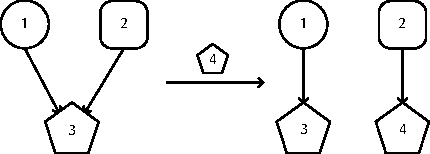
\includegraphics[width=\maxwidth{\textwidth}]{../img/react-references.pdf}
  \caption{Ukázka problému immutability a referencí}
  \label{fig:immutability-references}
\end{figure}

Problém s referencemi lze vyřešit tím, že každá odkazovaná třída v modelu bude mít datovou složku \texttt{id}, která bude instance unikátně identifikovat.
Potom instance jiných tříd budou referovat pomocí těchto složek.
Podobně je tomu například v relačních databázích.
Nevýhodou je, že může dojít ke dvěma nevalidním stavům: instance s daným \texttt{id} už neexistuje (např. byla smazána), nebo jich existuje více (došlo chybně k duplikaci objektu bez změny \texttt{id}).
Systém by se měl postarat o to, aby k tomu nedošlo.
Bohužel jsme se tímto připravili také o některé výhody, které v JavaScriptu poskytuje \acrfull{gc}.
Mezi objekty totiž referujeme způsobem, o kterém \acrshort{gc} nemůže vědět.

Když teď známe všechny restrikce na náš model, můžeme ho začít navrhovat.
Stejně jako pro konceptuální model k tomu použijeme \acrshort{uml} třídy s komentářem v textu.
Některé výše zmíněné povinné datové složky a atributy budeme v modelu považovat za implicitní.

Nebudeme popisovat úplně celý datový model kvůli jeho rozsahu.
Některé záležitosti, které se týkají pouze zobrazování nebo nejsou důležité ve více částech aplikace, vynecháme.

\begin{figure}[!htb]
  \centering
  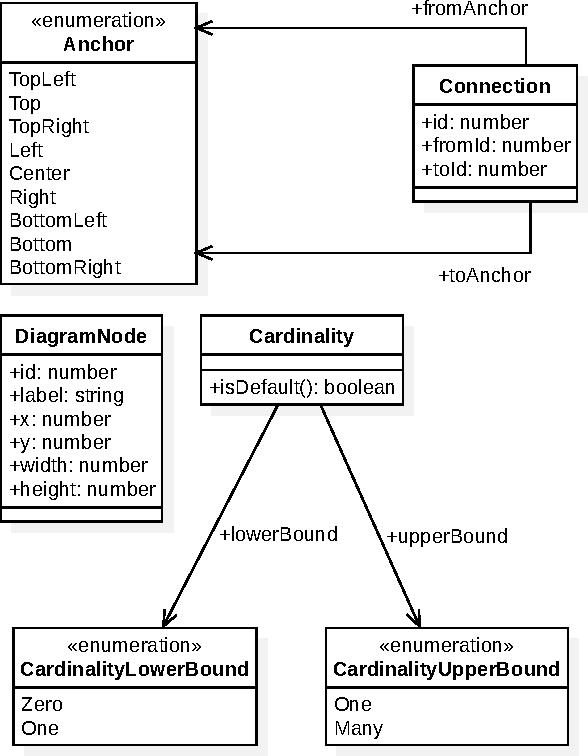
\includegraphics[width=\maxwidth{\textwidth}]{../img/diagrams/diagram-class-diagram.pdf}
  \caption{Diagram tříd -- diagram}
  \label{fig:diagram-class-diagram}
\end{figure}

Na Obrázku~\ref{fig:diagram-class-diagram} je diagram tříd popisující základní obecné konstrukty, které se týkají všech diagramů v systému.
Třída \texttt{Cardinality} obsahuje mj. operaci \texttt{isDefault}, která říká, zda se jedná o výchozí kardinalitu (námi definovanou jako \oneone).
V jazyce TypeScript, resp. JavaScript, nelze přetěžovat operátory, všechny operace musí být metody v dané třídě.
Dále v nich neexistuje koncept hodnotového porovnání instancí tříd, resp. porovnání objektů.
Pokud se porovnávají instance operátorem \texttt{==}, porovnávají se reference.

Z těchto důvodů nelze kardinalitu porovnat s jinou instancí bez přítomnosti odpovídající metody.
V našem případě je pouze potřeba zjistit, zda se jedná o výchozí kardinalitu, a proto definujeme odpovídající operaci.

Třída \texttt{Anchor} (kotva) se týká pouze zobrazení.
Říká, z a do které oblasti elementu diagramu vede odpovídající spojení.
Každý element diagramu si sám definuje a vypočítá těchto 9 kotev, které by se měly nacházet po jeho obvodu s výjimkou center.
Tyto kotvy jsou relativní k rozměrům a umístění elementu, a proto je musí vždy přepočítat.

Kvůli restrikci o více referencích má třída \texttt{DiagramNode} své \texttt{id}.
Toto bude běžné u většiny tříd, které reprezentují elementy diagramů.

\begin{figure}[!htb]
  \centering
  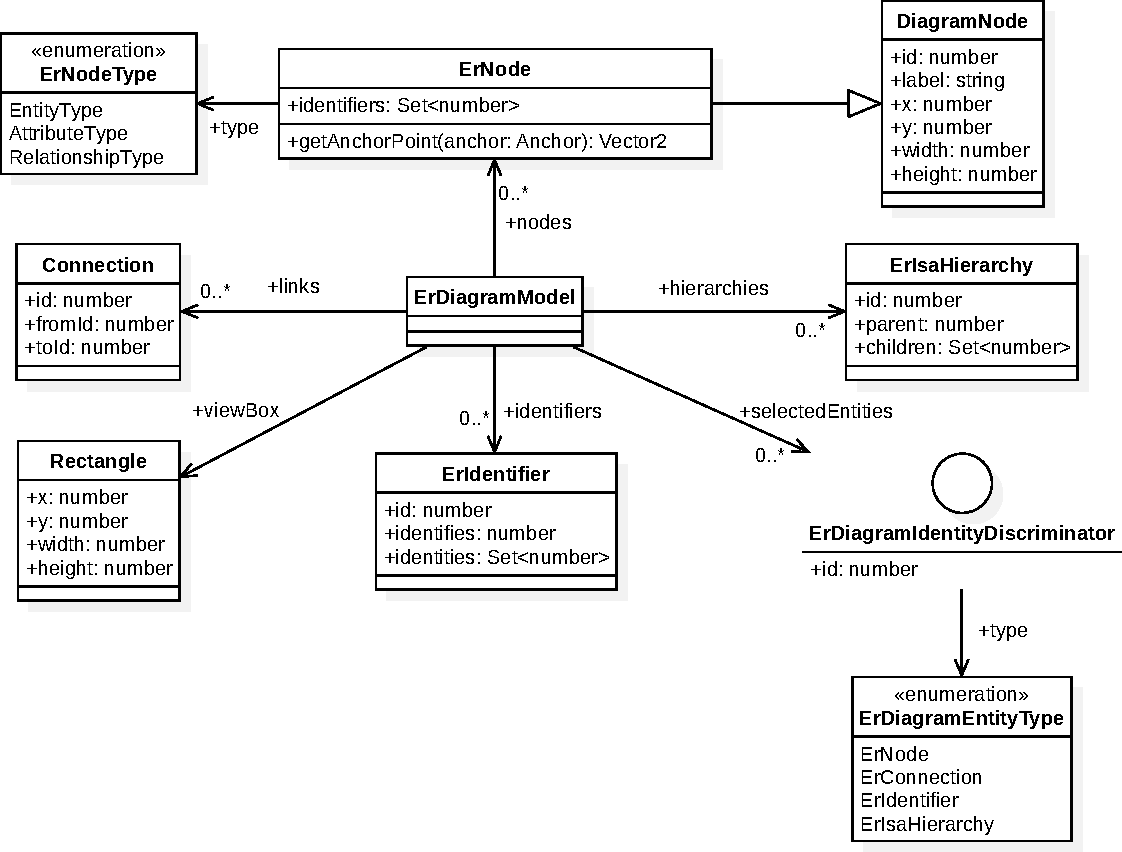
\includegraphics[width=\maxwidth{\textwidth}]{../img/diagrams/er-class-diagram.pdf}
  \caption{Diagram tříd -- \acrshort{er}}
  \label{fig:er-class-diagram}
\end{figure}

Na Obrázku~\ref{fig:er-class-diagram} je diagram tříd, které se týkají \acrshort{er} diagramu.

Hlavní třída \texttt{ErDiagramModel} je majitel svých \texttt{ErNode}, \texttt{Connection}, \texttt{ErIdentifier} a \texttt{ErIsaHierarchy}.
Pro zobrazování a uživatelskou interakci drží také rozhraní \texttt{ErDiagramIdentityDiscriminator}, které obaluje \texttt{id} uživatelem právě vybraných elementů diagramu.
Tento obal navíc obsahuje typový diskriminátor \texttt{type}, jenž vyjadřuje, o jaký druh elementu se jedná.
Tato typová diskriminace je důležitá, aby systém věděl, kde má daný element s daným \texttt{id} hledat, zdali mezi \texttt{nodes}, \texttt{links}, \texttt{identifiers}, nebo \texttt{hierarchies}.

Podobně je určen typ \texttt{ErNode}, který pro element diagramu říká, jak se má zobrazovat.
V \acrshort{er} jsme definoval tři hlavní elementy -- entitní typ, vztahový typ a atribut.
Mohli jsme tyto elementy modelovat jako jednotlivé třídy, ale tento přístup je vhodnější, protože rozdíl mezi nimi je pouze ve vizualizaci.
Také se tímto způsobem v jazyce TypeScrip jednodušeji pozná, o jaký typ má aktuálně držená instance \texttt{ErNode}.
V reakci na to lze jednodušeji implementovat v systému rozličnou logiku týkající se pouze jednotlivých typů elementů.

V diagramu používáme množinový typ \texttt{Set}, který je v JavaScriptu zabudovaný.
Jednodušeji se pak pracuje s odpovídajícími datovými složkami, kde nezáleží na pořadí a duplicitách.
Atributy \texttt{children} a \texttt{identities}, které tento typ mají, mají teoreticky kardinalitu \onemany{}.
V ISA hierarchii musí být alespoň jedno dítě a v identifikátoru alespoň jedna identita.

U třídy \texttt{ErIdentifier} bylo nutné názvem rozlišit jednotlivé datové složky.
Pojmenování může být matoucí, takže ho zde popíšeme.
Identifikátor (identifier) se skládá z jednoho entitního typu, jehož tímto identifikuje (identifies).
Součástí identifikátoru jsou pak jednotlivé elementy, ze kterých se identifikátor skládá.
Říkáme jim identity (identities).

Pro správné zobrazení diagramu má třída \texttt{ErDiagramModel} také datovou složku \texttt{viewBox}.
Ta vyjadřuje, na jakou část diagramu se má plátno zaměřit.
Jedná se o obdélník, který svou pozicí vyjadřuje přesun plátna a svou šířkou a výškou vyjadřuje přiblížení.
Třída \texttt{Rectangle} je obecná, a používá se proto i v jiných částech systému, kde je potřeba pracovat s obdélníky.


\begin{figure}[!htb]
  \centering
  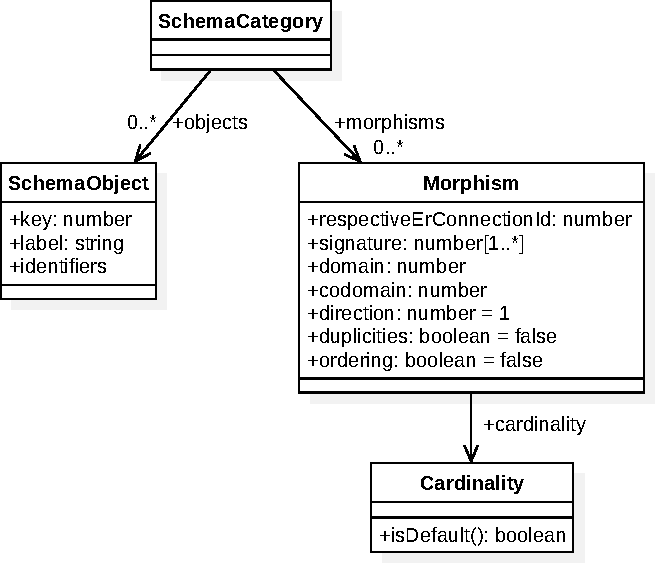
\includegraphics[width=\maxwidth{\textwidth}]{../img/diagrams/schemcat-class-diagram.pdf}
  \caption{Diagram tříd -- schematická kategorie}
  \label{fig:schemcat-class-diagram}
\end{figure}

Digram tříd, které se týkají schematické kategorie, je na Obrázku~\ref{fig:schemcat-class-diagram}.
Význam většiny obsahu tohoto diagramu je evidentní.
Upozorníme pouze na atribut \texttt{respectiveErConnectionId}.

Tento atribut vyjadřuje \texttt{id} \acrshort{er} spojení, z kterého daný morfismus vznikl.
Tato informace je užitečná pro aktualizaci morfismu v návaznosti na úpravu \acrshort{er} diagramu.
Také lze při úpravě schematické kategorie některé změny naopak převést zpět do \acrshort{er}.

Objekty schematické kategorie, které vznikly převodem z \acrshort{er} budou mít stejnou hodnotu \texttt{key} jako \texttt{id} odpovídajícího objektu.
Tím zaručíme stejnou svázanost diagramů jako tomu je u morfismů.

Dálě představíme vybrané třídy, které nesouvisí přímo s diagramy.
Pro práci s 2D geometrií budeme potřebovat třídy \texttt{Vector2} a \texttt{Angle}.

\begin{figure}[!htb]
  \centering
  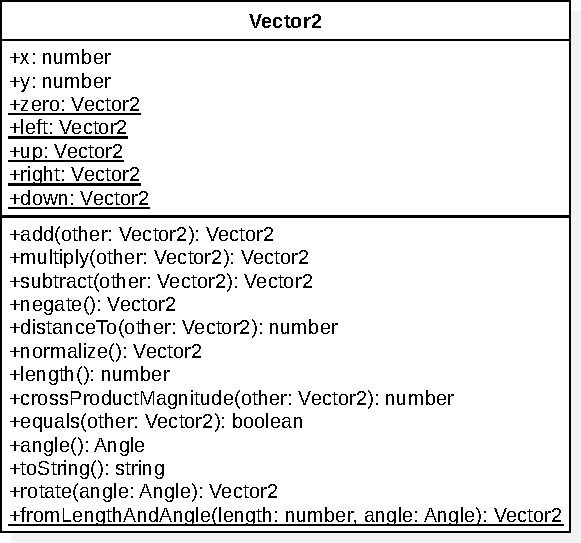
\includegraphics[width=\maxwidth{\textwidth}]{../img/diagrams/vector2-class-diagram.pdf}
  \caption{Diagram tříd -- \texttt{Vector2}}
  \label{fig:vector2-class-diagram}
\end{figure}

Třída \texttt{Vector2} z Obrázku~\ref{fig:vector2-class-diagram} reprezentuje dvourozměrný vektor s vhodnými operacemi včetně sčítání a odčítání s jinými vektory, násobení skalárem a negace (unární minus).
Další operace jsou vidět na zmíněném obrázku a jejich význam by měl být evidentní.
Třída poskytuje také běžně používané vektory jako statické atributy.
Operace, které pracují s úhly, používají k jejich reprezentaci třídu \texttt{Angle}.

\begin{figure}[!htb]
  \centering
  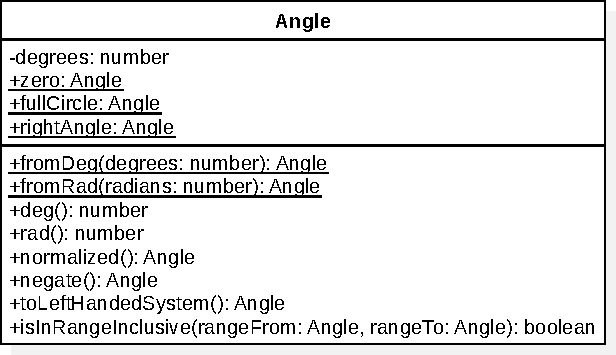
\includegraphics[width=\maxwidth{\textwidth}]{../img/diagrams/angle-class-diagram.pdf}
  \caption{Diagram tříd -- \texttt{Angle}}
  \label{fig:angle-class-diagram}
\end{figure}

Třída \texttt{Angle} z Obrázku~\ref{fig:angle-class-diagram} reprezentuje úhly nezávisle na jejich jednotkách.
Je to vhodnější, než používat pouze pomocné metody, které by převáděly stupně na radiány a naopak.
Interně je úhel reprezentován ve stupních, protože při počítání s radiány by kvůli menším číslům mohlo docházet ke ztrátě přesnosti.

Metoda \texttt{normalized} převede úhel do rozsahu $[0°, 360°)$, resp. $[0, 2\pi)$.
To jak pro negativní, tak pro pozitivní úhly mimo tyto rozsahy.

\begin{figure}[!htb]
  \centering
  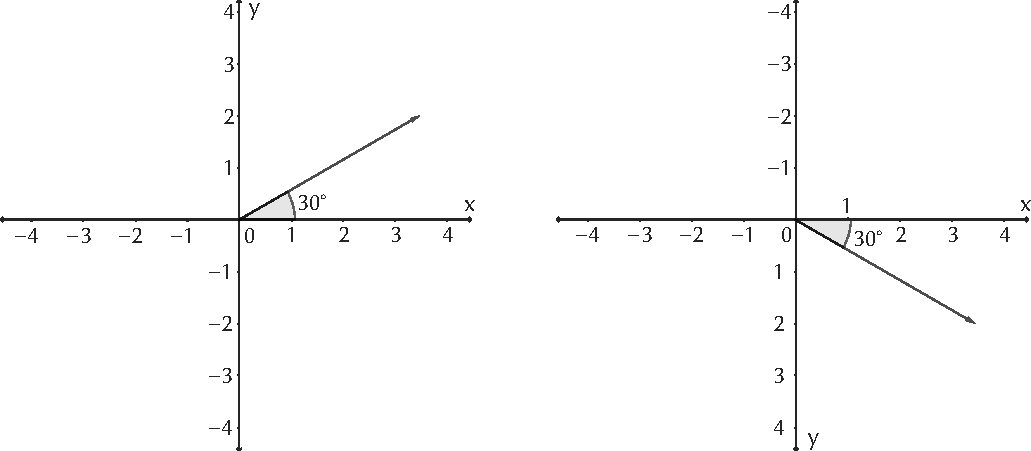
\includegraphics[width=\maxwidth{\textwidth}]{../img/cartesian-systems.pdf}
  \caption[Pravotočivá a levotočivá kartézská soustava souřadnic]{Pravotočivá (vlevo) a levotočivá (vpravo) kartézská soustava souřadnic}
  \label{fig:cartesian-systems}
\end{figure}

Na Obrázku~\ref{fig:cartesian-systems} jsou znázorněny dva typy kartézské soustavy souřadnic -- pravotočivá a levotočivá.
V matematice a geometrii je nejběžnější pravotočivá soustava souřadnic, nicméně \acrshort{svg} používá levotočivou (angl.~left-handed), jak je tomu běžné u počítačové grafiky.
Pro převod úhlu z běžně uvažovaného pravotočivého do levotočivého \acrshort{svg} úhlu slouží právě metoda \texttt{toLeftHandedSystem}.
Ta přijde vhod při rotování vektorů, či celých \acrshort{svg} konstruktů.

\begin{figure}[!htb]
  \centering
  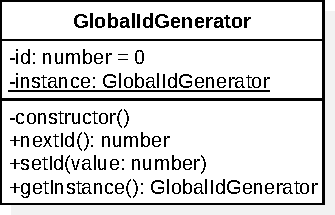
\includegraphics[width=\maxwidth{\textwidth}]{../img/diagrams/global-id-generator-class-diagram.pdf}
  \caption{Diagram tříd -- \texttt{GlobalIdGenerator}}
  \label{fig:global-id-gen-class-diagram}
\end{figure}

Třída \texttt{GlobalIdGenerator} z Obrázku~\ref{fig:global-id-gen-class-diagram} slouží jako generátor identifikátorů a klíčů pro naše objekty.
Zajišťuje, že vždy vrátí unikátní číslo jako nový identifikátor.
Jednoduchá implementace je začít s číslem 0 a každé další zvětšit o 1.
Tato třída je singleton, jeden z objektově orientovaných designových vzorů uvedený Gammou a kol. (také známých jako \enquote{Gang of Four})~\cite[s.~144]{gamma_designpatterns_1995}.
Tím může existovat nejvýše jedna její instance v běžícím systému.

\begin{figure}[!htb]
  \centering
  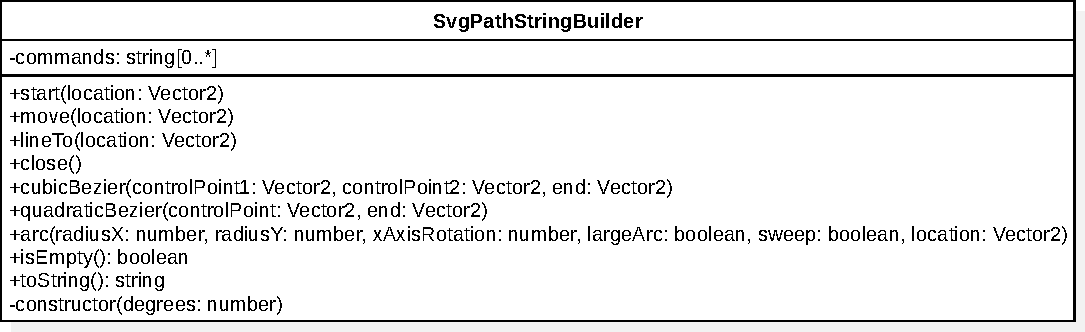
\includegraphics[width=\maxwidth{\textwidth}]{../img/diagrams/svg-path-string-builder-class-diagram.pdf}
  \caption{Diagram tříd -- \texttt{SvgPathStringBuilder}}
  \label{fig:svg-path-string-builder-class-diagram}
\end{figure}

Třída \texttt{SvgPathStringBuilder} z Obrázku~\ref{fig:svg-path-string-builder-class-diagram} konstruuje \acrshort{svg} path data atribut \cite[\S~9.3]{brinza_svg_2018}.
Obsahuje mnoho dalších metod.
Kromě těch, které lze vidět na zmíněném obrázku, například pro každý příkaz lze pozice (location) specifikovat i relativně k předchozí pozici (místo absolutně).
Třída odpovídá vzoru builder~\cite[s.~110]{gamma_designpatterns_1995}.
Užívání této třídy odpovídá vypisování \enquote{příkazů} pro path data atribut.
Užitečnost této třídy spočívá v přehlednosti -- je lepší používat její metody s deskriptivním názvem místo path data příkazů, které mají formu jednoho písmene a argumentů.

\section{Scénáře}

V této sekci uvedeme scénáře pro případy užití~\cite[s.~65]{overgaard_usecases_2005}, kterými rozšíříme procesy.

Případy užití nebudeme popisovat všechny, kvůli stručnosti.
Navíc některé případy užití jsou si velmi podobné, například export do \acrshort{svg} je téměř stejný jako export do \acrshort{png}, akorát se u \acrshort{svg} nevolí barva pozadí.
Zvolíme tedy pouze případy užití, které jsou nějak modelové nebo zásadní.

\begin{figure}[!htb]
  \centering
  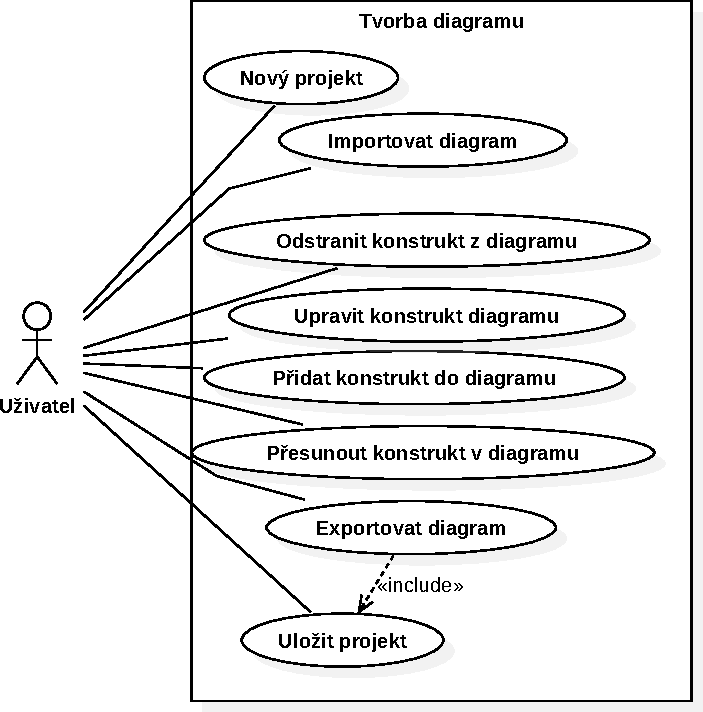
\includegraphics[width=\maxwidth{0.7\textwidth}]{../img/diagrams/use-case-diagram.pdf}
  \caption{Diagram případů užití}
  \label{fig:use-case-diagram}
\end{figure}

\newcommand{\ucsub}[1]{\textbf{#1}}
\newcommand{\uc}[1]{\subsection*{#1}}
\def\ucstart{\ucsub{Počáteční stav: }}
\def\ucnormal{\ucsub{Běžný průběh:}}
\def\ucerrors{\ucsub{Možné chyby:}}
\def\ucend{\ucsub{Stav systému po dokončení: }}

\uc{Modelování entitního typu v \acrshort{er} diagramu}
\ucstart{}
V systému je rozdělaný projekt.
\acrshort{er} diagram lze editovat.

\ucnormal{}
\begin{enumerate}
  \item Uživatel přetáhne myší konstrukt \enquote{entitní typ} z panelu konstruktů do \acrshort{er} diagramu.
  \item V diagramu je vytvořen nový entitní typ s výchozím názvem.
  \item Uživatel zvolí právě vytvořený entitní typ myší.
  \item V panelu \enquote{Control Panel} upraví vlastnost entitního typu \enquote{label}.
  \item Název entitního typu se změní na uživatelem definovaný.
\end{enumerate}

\ucend{}
V diagramu je nový entitní typ, který má uživatelem definovaný název.
Změna se projeví i ve schematické kategorii, respektive v její vizualizaci.

\uc{Modelování vztahového typu v \acrshort{er} diagramu}
\ucstart{}
V diagramu je entitní typ nebo více entitních typů, které se budou účastnit vztahového typu.
Případně je lze vytvořit i v průběhu toho případu užití.
Změna se projeví i ve schematické kategorii, resp. v její vizualizaci.

\ucnormal{}
\begin{enumerate}
  \item Uživatel z panelu s konstrukty myší přetáhne vztahový typ do \acrshort{er} diagramu.
  \item V \acrshort{er} diagramu se objeví nový vztahový typ.
  \item Uživatel v ovládacím panelu změní název vztahového typu.
  \item Uživatel spojí entitní typ se vztahovým typem podle už popsaného případu užití spojování elementů. Tím přidá účastníka vztahového typu.
  \item To zopakuje s dalšími účastníky (ne nutně jinými).
\end{enumerate}

\ucend{}
V systému je nyní nový vztahový typ s účastníky. To se projeví i ve schematické kategorii, resp. v její vizualizaci.

\uc{Modelování atributu v \acrshort{er} diagramu}
\ucstart{}
V \acrshort{er} diagramu je entitní typ. Diagram lze editovat.

\ucnormal{}
\begin{enumerate}
  \item Uživatel pravým tlačítkem myši klikne na entitní typ nebo vztahový typ.
  \item Otevře se kontextové menu.
  \item Uživatel zvolí položku \enquote{Add attribute}.
  \item Do \acrshort{er} diagramu je přidán nový atribut, který je spojen s entitním typem.
  \item Uživatel zvolí právě vytvořený atribut myší.
  \item V ovládacím panelu upraví vlastnost \enquote{label}.
  \item Název atributu je nastaven na právě uživatelem definovaný.
  \item Uživatel případně zvolí spojení mezi entitním typem a atributem myší.
  \item V ovládacím panelu zvolí kardinalitu ze čtyř předdefinovaných možností.
  \item Tato kardinalita je pro spojení nastavena.
\end{enumerate}

\ucend{}
V modelu systému je uložen nový atribut entitního typu, který má daný název a kardinalitu.
Změna se projeví i ve schematické kategorii, resp. v její vizualizaci.

\uc{Přidání spojení mezi dva \acrshort{er} elementy diagramu}
\ucstart{}
V \acrshort{er} diagramu dva existující elementy.

\ucnormal{}
\begin{enumerate}
  \item Uživatel zvolí první element levým tlačítkem myši.
  \item Uživatel klikne na druhý element pravým tlačítkem myši.
  \item Zobrazí se kontextové menu.
  \item Uživatel zvolí položku \enquote{New connection}.
  \item Mezi elementy se vloží spojení.
\end{enumerate}

\ucerrors{}
\begin{itemize}
  \item Elementy mohou být nekompatibilní -- např. dva vztahové typy, dva entitní typy.
        V takovém případě se spojení nevytvoří a zobrazí se chybová hláška.
\end{itemize}

\ucend{}
V modelu i v zobrazeném diagramu bude mezi elementy nové spojení.

\uc{Export libovolného diagramu do \acrshort{png}}
\ucstart{}
V systému je otevřený projekt.

\ucnormal{}
\begin{enumerate}
  \item Uživatel zvolí položku \menu{File > Export as > PNG} v hlavním menu aplikace.
  \item Otevře se dialog s možnostmi exportu s výběrem diagramu k exportu. Výchozí zvolený diagram bude ten, ve kterém naposledy uživatel pracoval.
  \item V dialogu dále uživatel zvolí, jestli chce do \acrshort{png} souboru zahrnout i serializovanou verzi projektu, aby šel později \acrshort{png} soubor otevřít v aplikaci.
  \item Uživatel v dialogu dále zvolí, jestli má \acrshort{png} mít barvu pozadí, případně jakou. Výchozí nastavení je \acrshort{png} bez pozadí, tedy transparentní.
  \item Uživatel potvrdí dialog.
  \item V prohlížeči uživatele se \enquote{stáhne} exportovaný \acrshort{png} soubor, který má název odpovídající názvu projektu.
\end{enumerate}

\ucerrors{}
\begin{itemize}
  \item V zařízení uživatele není dostatek persistentní paměti na uložení obrázku.
        O zachycení a obstarání této chyby se stará webový prohlížeč uživatele.
  \item Soubor se stejným názvem již existuje.
        O zachycení a obstarání se rovněž stará webový prohlížeč uživatele.
  \item Uživatel zruší dialog místo potvrzení. V takovém případě se nic dalšího nestane (nedojde k exportu).
\end{itemize}

\ucend{}
Ve složce nastavené ve webovém prohlížeči uživatele na uložení stahovaných souborů bude uložen \acrshort{png} soubor s rasterizovaným diagramem.

% \chapter*{Závěr}
\addcontentsline{toc}{chapter}{Závěr}

Závěr

%%% Seznam použité literatury
%%% Seznam použité literatury (bibliografie)
%%%
%%% Pro vytváření bibliografie používáme bibTeX. Ten zpracovává
%%% citace v textu (např. makro \cite{...}) a vyhledává k nim literaturu
%%% v souboru literatura.bib.
%%%
%%% Příkaz \bibliographystyle určuje, jakým stylem budou citovány odkazy
%%% v textu. V závorce je název zvoleného souboru .bst. Styly plainnat
%%% a unsrt jsou standardní součástí latexových distribucí. Styl czplainnat
%%% je dodáván s touto šablonou a bibTeX ho hledá v aktuálním adresáři.

% \bibliographystyle{czplainnat}    %% Autor (rok) s českými spojkami
% \bibliographystyle{plainnat}    %% Autor (rok) s anglickými spojkami
% \bibliographystyle{unsrt}       %% [číslo], unsorted
\bibliographystyle{unsrturl}       %% [číslo], unsorted + url support

\renewcommand{\bibname}{Seznam použité literatury}

%%% Vytvoření seznamu literatury. Pozor, pokud jste necitovali ani jednu
%%% položku, seznam se automaticky vynechá.

\bibliography{literatura}

%%% Kdybyste chtěli bibliografii vytvářet ručně (bez bibTeXu), lze to udělat
%%% následovně. V takovém případě se řiďte normou ISO 690 a zvyklostmi v oboru.

% \begin{thebibliography}{99}
%
% \bibitem{lamport94}
%   {\sc Lamport,} Leslie.
%   \emph{\LaTeX: A Document Preparation System}.
%   2. vydání.
%   Massachusetts: Addison Wesley, 1994.
%   ISBN 0-201-52983-1.
%
% \end{thebibliography}


%%% Obrázky v bakalářské práci
%%% (pokud jich je malé množství, obvykle není třeba seznam uvádět)
\listoffigures

%%% Tabulky v bakalářské práci (opět nemusí být nutné uvádět)
%%% U matematických prací může být lepší přemístit seznam tabulek na začátek práce.
\listoftables

%%% Použité zkratky v bakalářské práci (opět nemusí být nutné uvádět)
%%% U matematických prací může být lepší přemístit seznam zkratek na začátek práce.

% \chapwithtoc{Seznam použitých zkratek}

%%% Přílohy k bakalářské práci, existují-li. Každá příloha musí být alespoň jednou
%%% odkazována z vlastního textu práce. Přílohy se číslují.
%%%
%%% Do tištěné verze se spíše hodí přílohy, které lze číst a prohlížet (dodatečné
%%% tabulky a grafy, různé textové doplňky, ukázky výstupů z počítačových programů,
%%% apod.). Do elektronické verze se hodí přílohy, které budou spíše používány
%%% v elektronické podobě než čteny (zdrojové kódy programů, datové soubory,
%%% interaktivní grafy apod.). Elektronické přílohy se nahrávají do SISu a lze
%%% je také do práce vložit na CD/DVD. Povolené formáty souborů specifikuje
%%% opatření rektora č. 72/2017.

% \appendix
% \chapter{Přílohy}

% \section{První příloha}

\openright
\end{document}
